\documentclass[14pt]{extarticle}

\usepackage{fontspec}
\setmainfont{Times New Roman}

% размер полей
\usepackage{geometry}
\geometry{a4paper, top=2cm, bottom=2cm, right=1.5cm, left=3cm}

 %debugging
%\usepackage{showframe}

% полуторный интервал
\usepackage{setspace}
\onehalfspacing

% абзацный отступ
\setlength{\parindent}{1.25cm}

% выравнивание текста по ширине
\sloppy

% списки
\usepackage{calc} % арифметические операции с величинами
\usepackage{enumitem}
\setlist{
    nosep,
    leftmargin=0pt,
    itemindent=\parindent + \labelwidth - \labelsep,
}

% подписи к рисункам и таблицам
\usepackage{caption}
\renewcommand{\figurename}{Рисунок}
\renewcommand{\tablename}{Таблица}
\DeclareCaptionFormat{custom}
{
    \textit{#1#2#3}
}
\DeclareCaptionLabelSeparator{custom}{. }
\captionsetup{
    % хз какой это размер - 12 или нет, но выглядит меньше 14
    font=small,
    format=custom,
    labelsep=custom,
}

% картинки
\usepackage{graphicx}

% колонтитулы
\usepackage{fancyhdr}

% картинки и таблицы находятся именно в том месте текста где помещены (атрибут H)
\usepackage{float}

% таблицы
\usepackage{tabularray}

\graphicspath{ {6.3.1/models/} }
\begin{document}
\pagestyle{fancy}
\fancyhead{}
% disable header
\renewcommand{\headrulewidth}{0pt}
\fancyfoot[L]{Дубровских гр 221-361}
\fancyfoot[C]{ЛР 6.3.1}
\fancyfoot[R]{Продажа автотранспорта}
\singlespacing

\newpage
\begin{center}
    Министерство науки и высшего образования Российской Федерации
    Федеральное государственное автономное образовательное учреждение

    высшего образования

    \guillemotleft МОСКОВСКИЙ ПОЛИТЕХНИЧЕСКИЙ УНИВЕРСИТЕТ\guillemotright

    (МОСКОВСКИЙ ПОЛИТЕХ)
\end{center}
\noindent
\bigbreak
\bigbreak
\bigbreak
\bigbreak
\begin{center}
    ЛАБОРАТОРНАЯ РАБОТА 6.3.1

    По курсу Проектирования пользовательских интерфейсов в веб

    \textbf{Анализ цветового решения сайтов с учетом аномалий цветового восприятия}
    \bigbreak
    \bigbreak
    \bigbreak
    \bigbreak
    ТЕМА

    \guillemotleft\textbf{САЙТ ДЛЯ ПРОДАЖИ И ПОИСКА АВТОМОБИЛЕЙ}\guillemotright
\end{center}
\noindent
\bigbreak
\bigbreak
\bigbreak
\bigbreak
\bigbreak
\bigbreak
\bigbreak
\bigbreak
\bigbreak
\bigbreak
\hfill Выполнил

\hfill Дубровских Никита Евгеньевич

\hfill Группа 221-361
\bigbreak
\bigbreak
\bigbreak
\hfill Проверил

\hfill Натур ВВ
\vfill
\begin{center}
    Москва, 2024
\end{center}
\newpage
\onehalfspacing


\begin{center}
    \textbf{Лабораторная работа 6.3.1}

    \textbf{Анализ цветового решения сайтов с учетом аномалий цветового восприятия}
\end{center}

\textbf{Цель работы:} проанализировать цветовое решение сайтов с позиции сохранения контраста элементов при просмотре людьми с различными расстройствами цветового восприятия.
\bigskip

\textbf{Задачи:}

\begin{enumerate}
    \item Изучить критерии и принципы цветового решения сайтов с позиции сохранения контраста элементов.
    \item Изучить аномалии цветового восприятия пользователей. 
    \item Проанализировать рекомендации по проектированию интерфейса сайта (моб. приложения) с учетом аномалий цветового восприятия пользователей.
    \item Познакомиться с международным стандартом Web Content Accessibility Guidelines (пер. «Руководство по доступности веб-материалов») - WCAG.
\end{enumerate}
\bigskip

\textbf{Основные термины}

\begin{itemize}
    \item Аномалии цветового восприятия – различные формы нарушения восприятия цветов, включая цветовую слабость и цветовую слепоту, которые могут быть врожденными или приобретенными. Важны для учета при разработке интерфейсов для доступности.
    \item Цветовая слепота (дальтонизм) – неспособность различать определенные цвета из-за дисфункции одного из типов колбочек. Различные типы дальтонизма, такие как протанопия, дейтеранопия и тританопия, требуют особого подхода к выбору цветовых решений.
    \item Цветовая слабость – частичное нарушение восприятия одного из основных цветов (красного, зеленого или синего). Этот тип аномалии встречается чаще, чем цветовая слепота, и нуждается в особом подходе к контрастности интерфейсов.
    \item Web Content Accessibility Guidelines (WCAG) – международный стандарт, регламентирующий доступность веб-контента для людей с ограниченными возможностями, включая людей с нарушениями зрения. Описание критериев и рекомендаций WCAG помогает дизайнерам создавать более доступные интерфейсы.
    \item Контрастность – степень различимости элементов интерфейса, ключевая для обеспечения читаемости и восприятия элементов пользователями с нарушениями цвета. Высокий контраст помогает улучшить восприятие для людей с дальтонизмом.
    \item Симулятор цветовых аномалий – программное обеспечение (например, Colorfilter или Coblis), которое показывает, как интерфейсы выглядят для людей с различными типами дальтонизма. Используется для тестирования и корректировки цветового решения сайтов.
\end{itemize}
\bigskip

\textbf{Анализ цветового решения сайта с учетом аномалий цветового восприятия}

\begin{enumerate}
    \item Используйте и цвет и символы

Не нужно полагаться только на цвет, чтобы передать сообщение. Например, некоторые типы цветовой слепоты могут затруднить или даже вообще не позволить человеку увидеть общие красные сообщения об ошибках. Один из подходов заключается в использовании как цветов, так и символов, требующих внимания пользователя.

\noindent
\begin{minipage}{\linewidth}
    \fbox{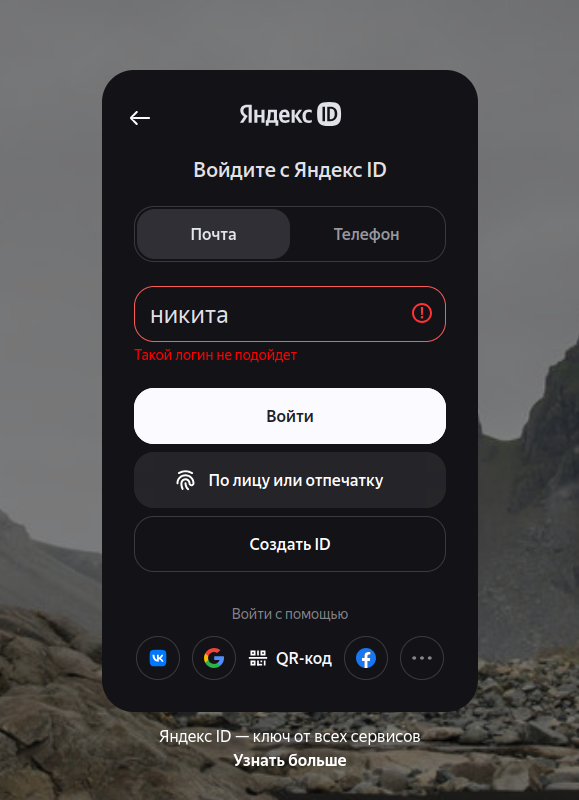
\includegraphics[width=\linewidth]{color_symbol}}
    \captionof{figure}{passport.yandex.ru/auth}
\end{minipage}
\bigskip

\item Соблюдайте минимализм

    Вы должны ограничить цветовую палитру, которую вы используете для своего сайта. Чем меньше цветов вы используете в своем дизайне, тем меньше будет возможностей для создания путаницы.

\noindent
\begin{minipage}{\linewidth}
    \fbox{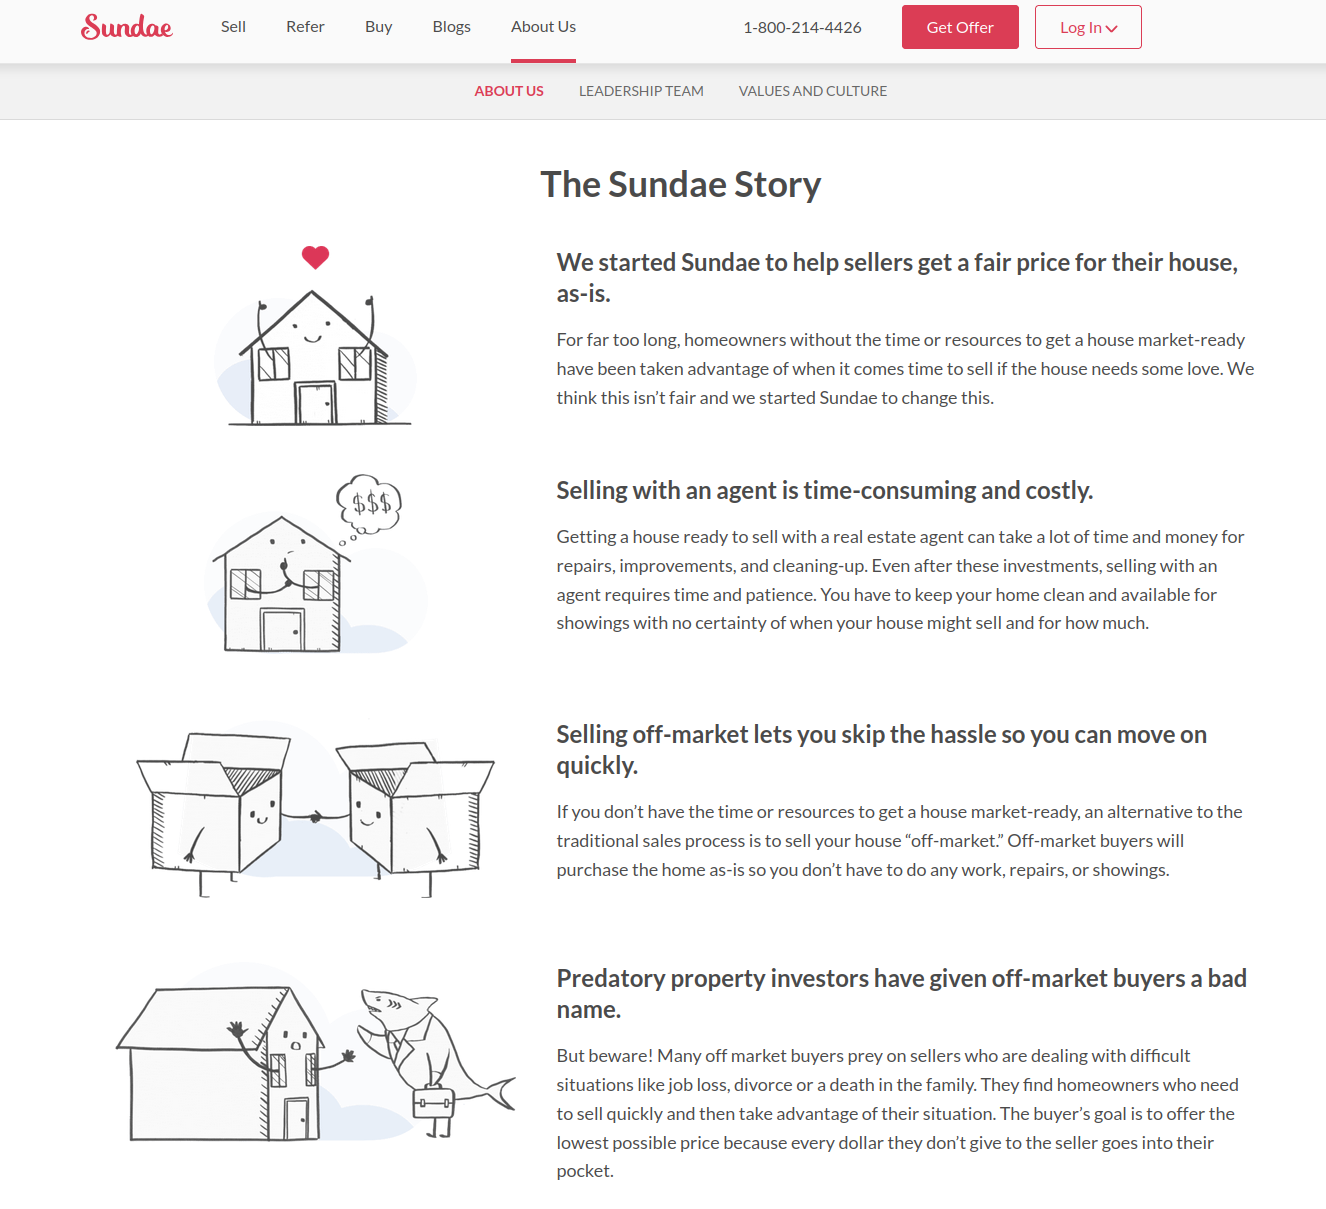
\includegraphics[width=\linewidth]{minimalism}}
    \captionof{figure}{sundae.com/about-us}
\end{minipage}
\bigskip

\noindent
\begin{minipage}{\linewidth}
    \fbox{
\includegraphics[width=\linewidth]{minimalism2}}
    \captionof{figure}{valuemont.com}
\end{minipage}
\bigskip

\item Используйте паттерны и текстуры

Попытайтесь использовать разные текстуры вместо нескольких цветов для элементов, которые требуют внимания. Например, может быть трудно для слепых пользователей интерпретировать графики и диаграммы. В этом случае лучше использовать контрастные шаблоны и, если возможно, разместить текст.

\noindent
\begin{minipage}{\linewidth}
    \fbox{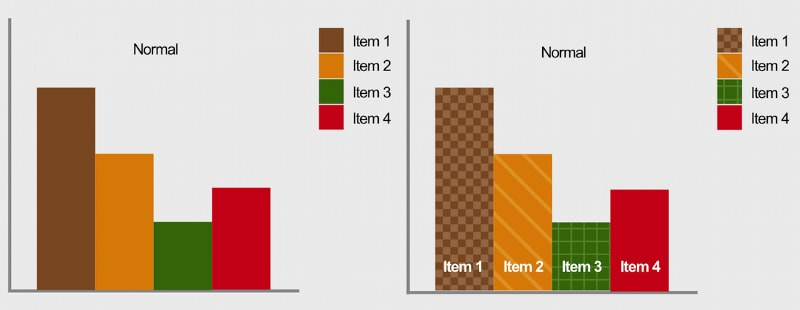
\includegraphics[width=\linewidth]{texture}}
\end{minipage}
\bigskip

\item Будьте осторожны с цветовым контрастом и насыщенностью

Вместо того, чтобы полагаться на черно-белое, как на ваши единственные контрастные цвета, попробуйте использовать ряд контрастных цветов и оттенков в вашем дизайне. Например, игра 2048 использует различные контрастные цвета для своих плиток, которые можно легко отличить друг от друга вне зависимости от того, есть у человека дальтонизм или нет.

\noindent
\begin{minipage}{\linewidth}
    \fbox{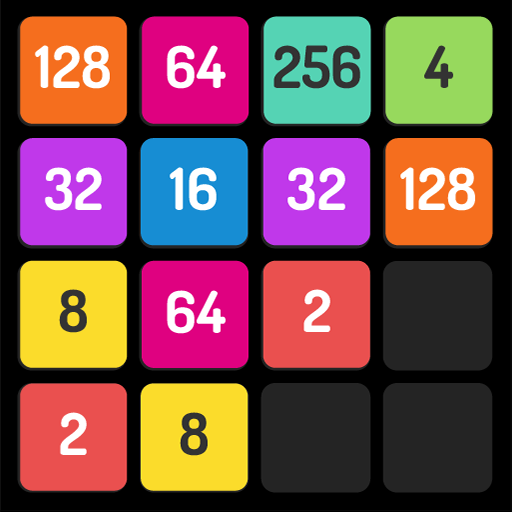
\includegraphics[width=\linewidth]{contrast}}
    \captionof{figure}{Игра 2048}
\end{minipage}
\bigskip

\item Избегайте плохой цветовой пары

    \begin{itemize}
        \item красный – зеленый
        \item зеленый – коричневый
        \item голубой – пурпурный
        \item голубой – зеленый
        \item салатовый – желтый
        \item голубой – серый
        \item зеленый – серый
        \item зеленый – черный
    \end{itemize}

\end{enumerate}
\bigskip

Использование правильных цветовых комбинаций.

Выбор правильных цветовых комбинаций для текста и фона может помочь обеспечить хорошую контрастность. Например, черный текст на белом фоне обычно обеспечивает высокую контрастность.
Ниже представлен скриншот с сайтом  avito.ru, на котором можно увидеть различия в цветах между нормальным восприятием и восприятием с протанопией (проблемы с красным цветом), а также с ахроматопсией - человек различает цвета только по их яркости.
\bigskip

\noindent
\begin{minipage}{\linewidth}
    \fbox{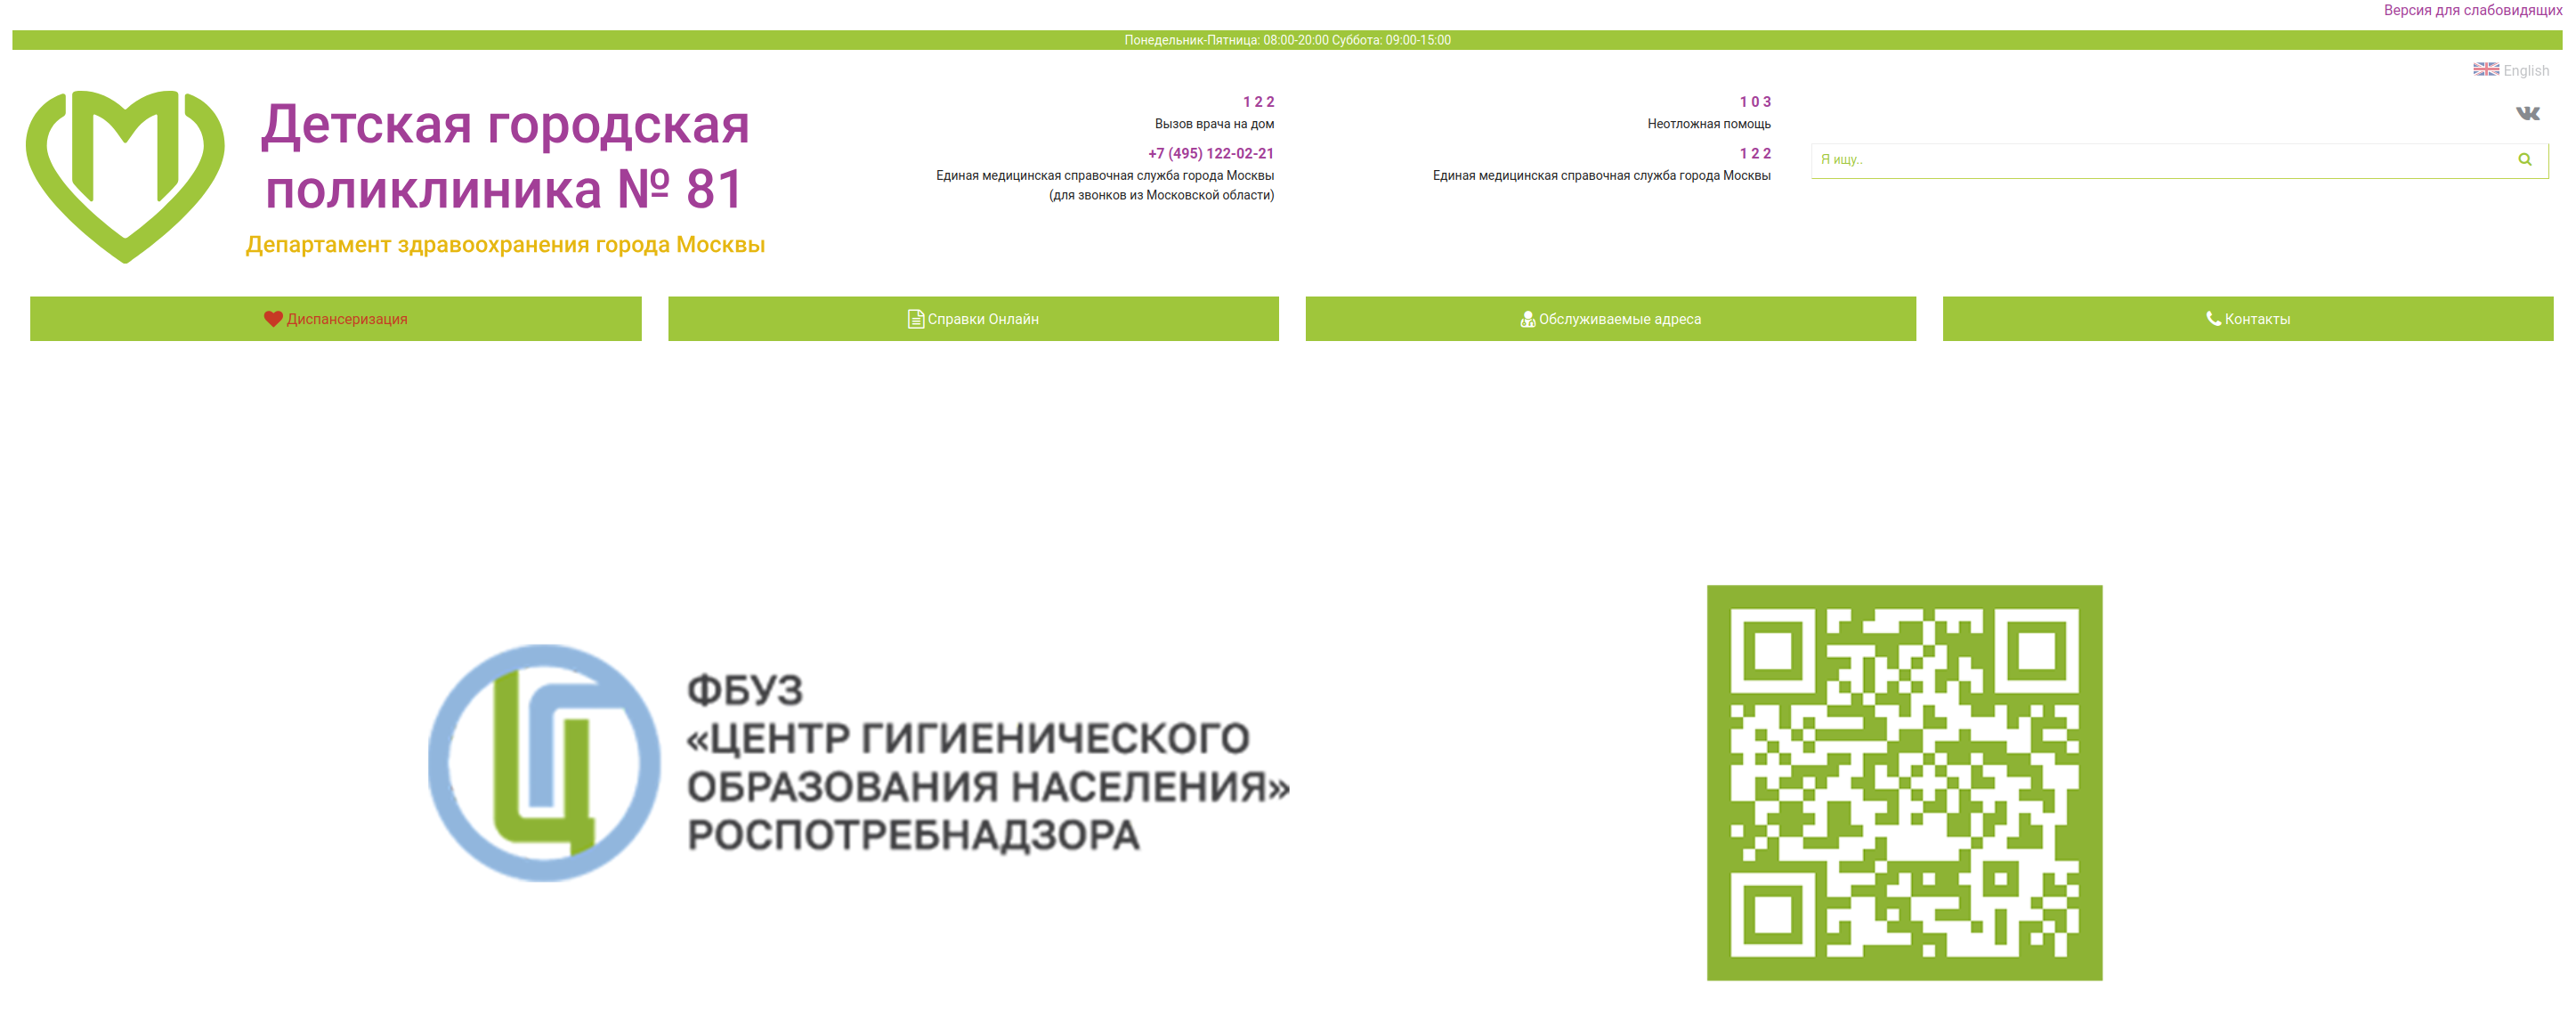
\includegraphics[width=\linewidth]{81}}
    \captionof{figure}{dgp81.mos.ru}
\end{minipage}
\bigskip

\noindent
\begin{minipage}{\linewidth}
    \fbox{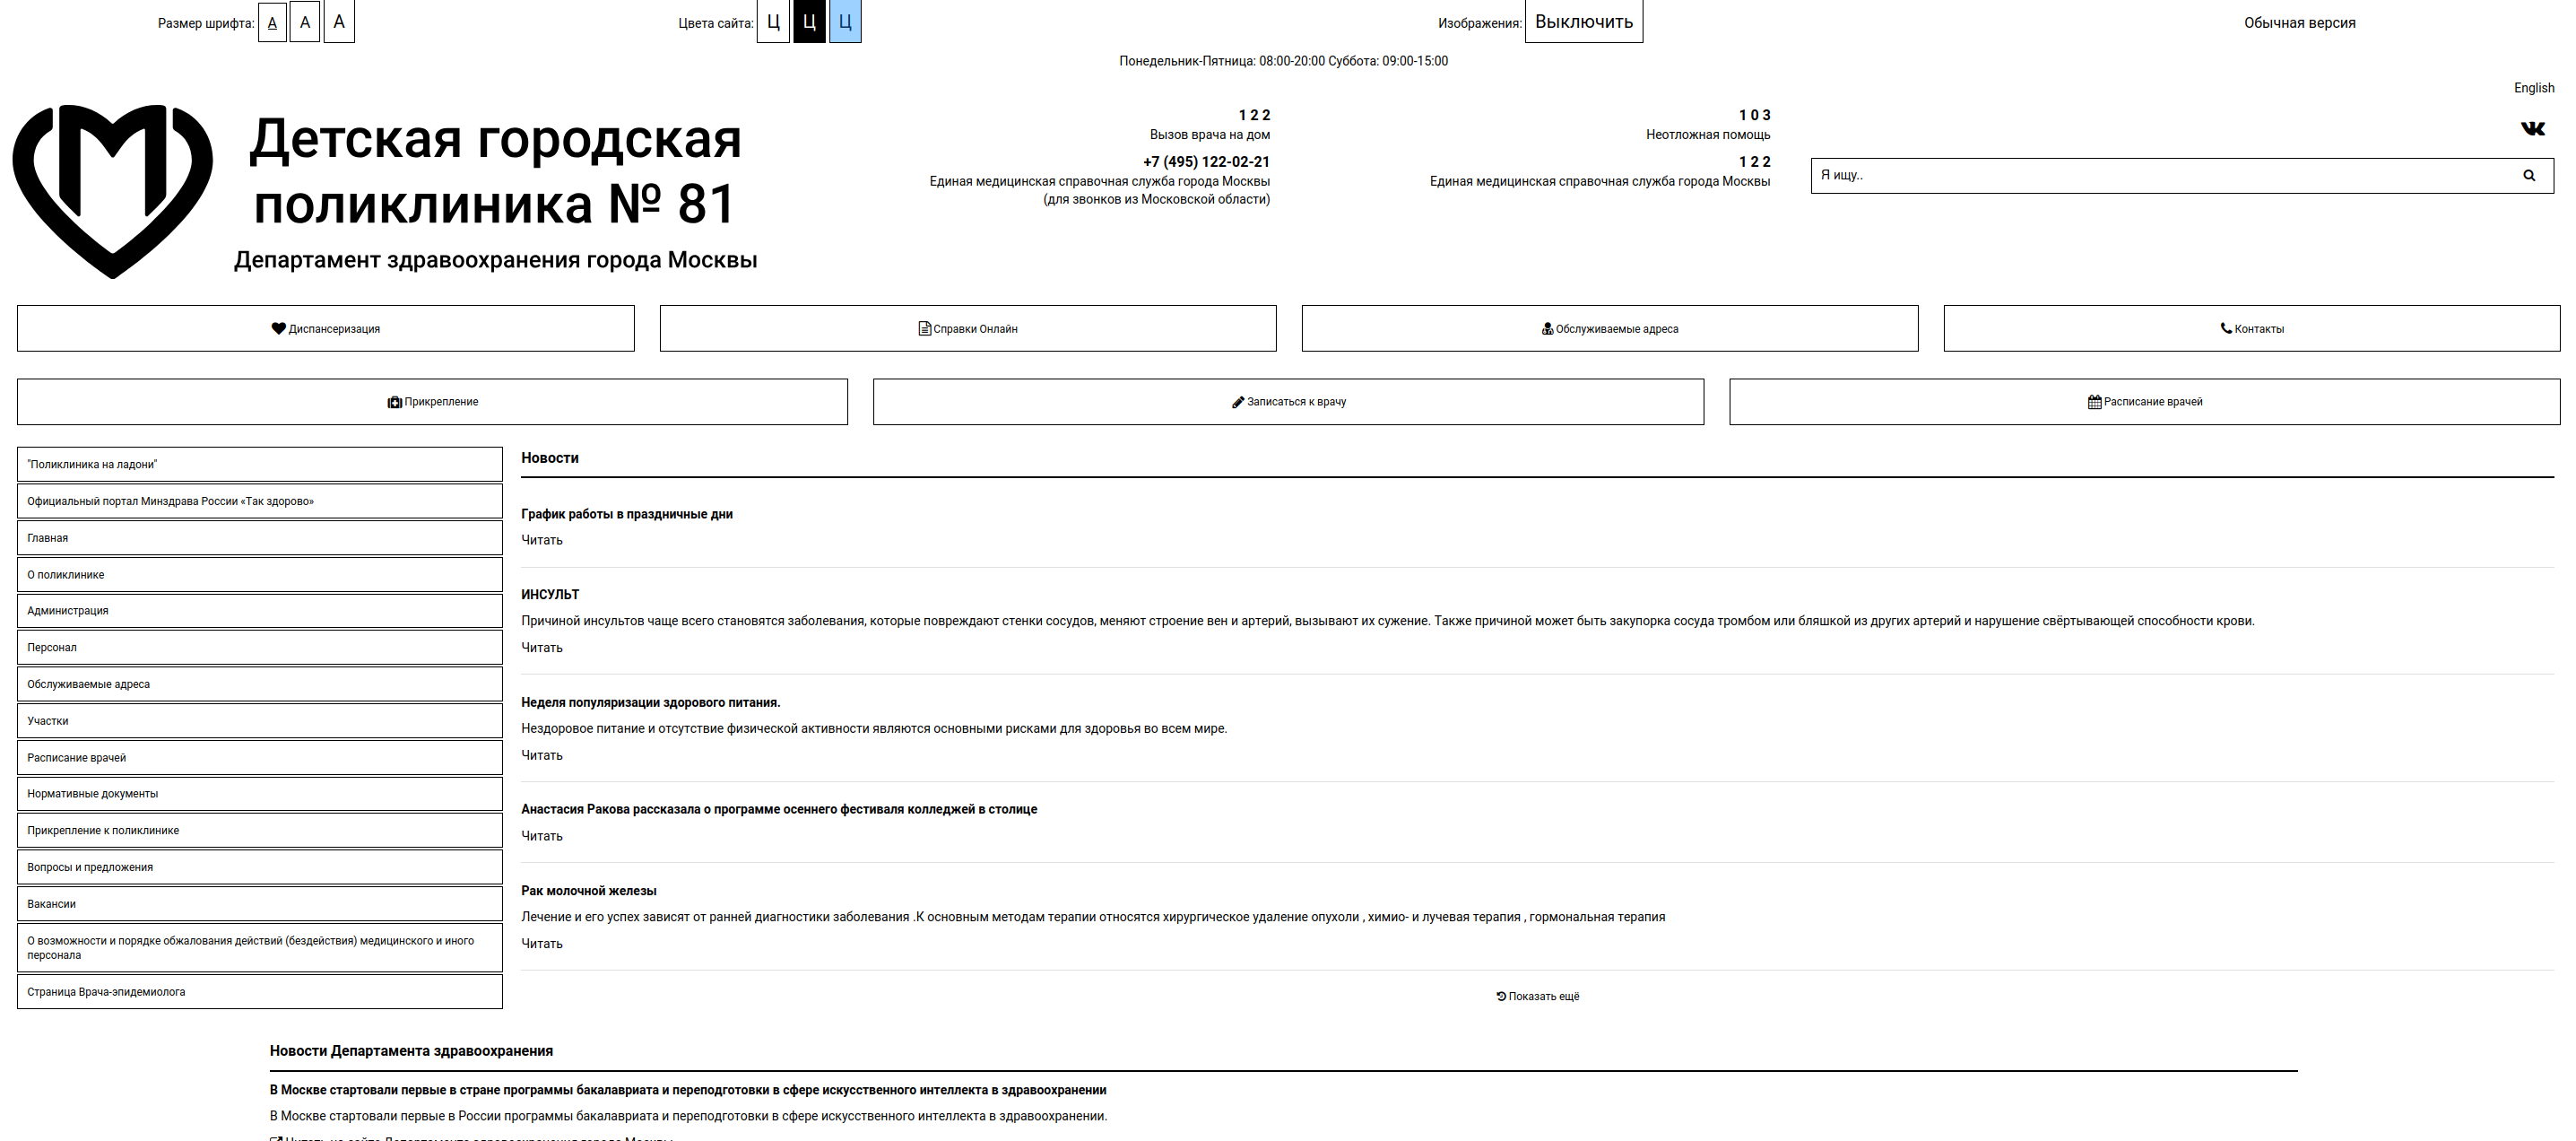
\includegraphics[width=\linewidth]{81_2}}
    \captionof{figure}{dgp81.mos.ru версия для слабовидящих}
\end{minipage}
\bigskip

\noindent
\begin{minipage}{\linewidth}
    \fbox{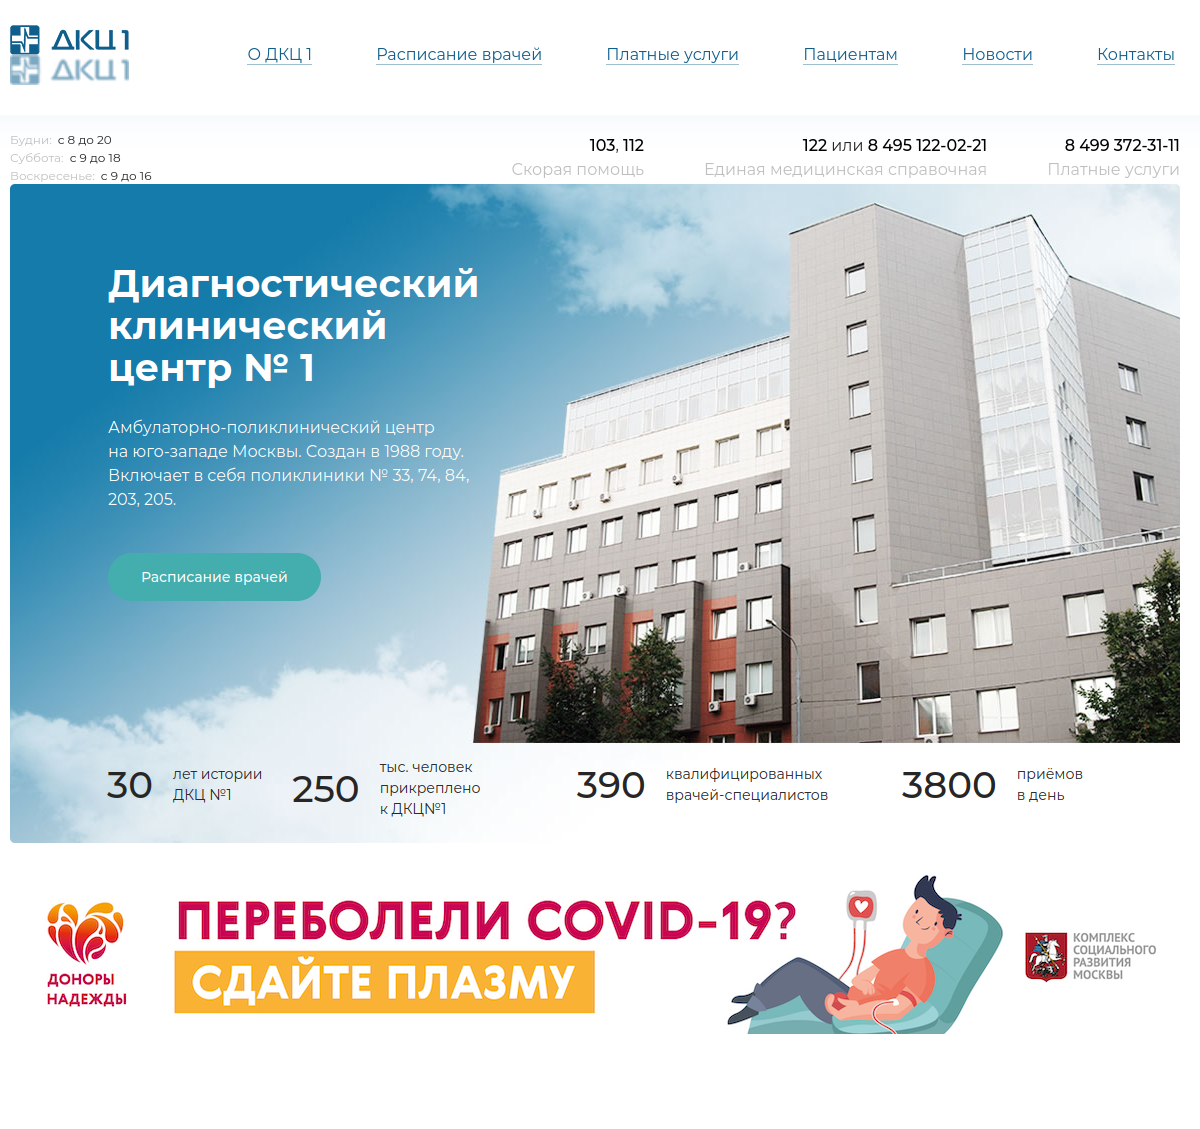
\includegraphics[width=\linewidth]{dkz1}}
    \captionof{figure}{дкц1.рф}
\end{minipage}
\bigskip

\noindent
\begin{minipage}{\linewidth}
    \fbox{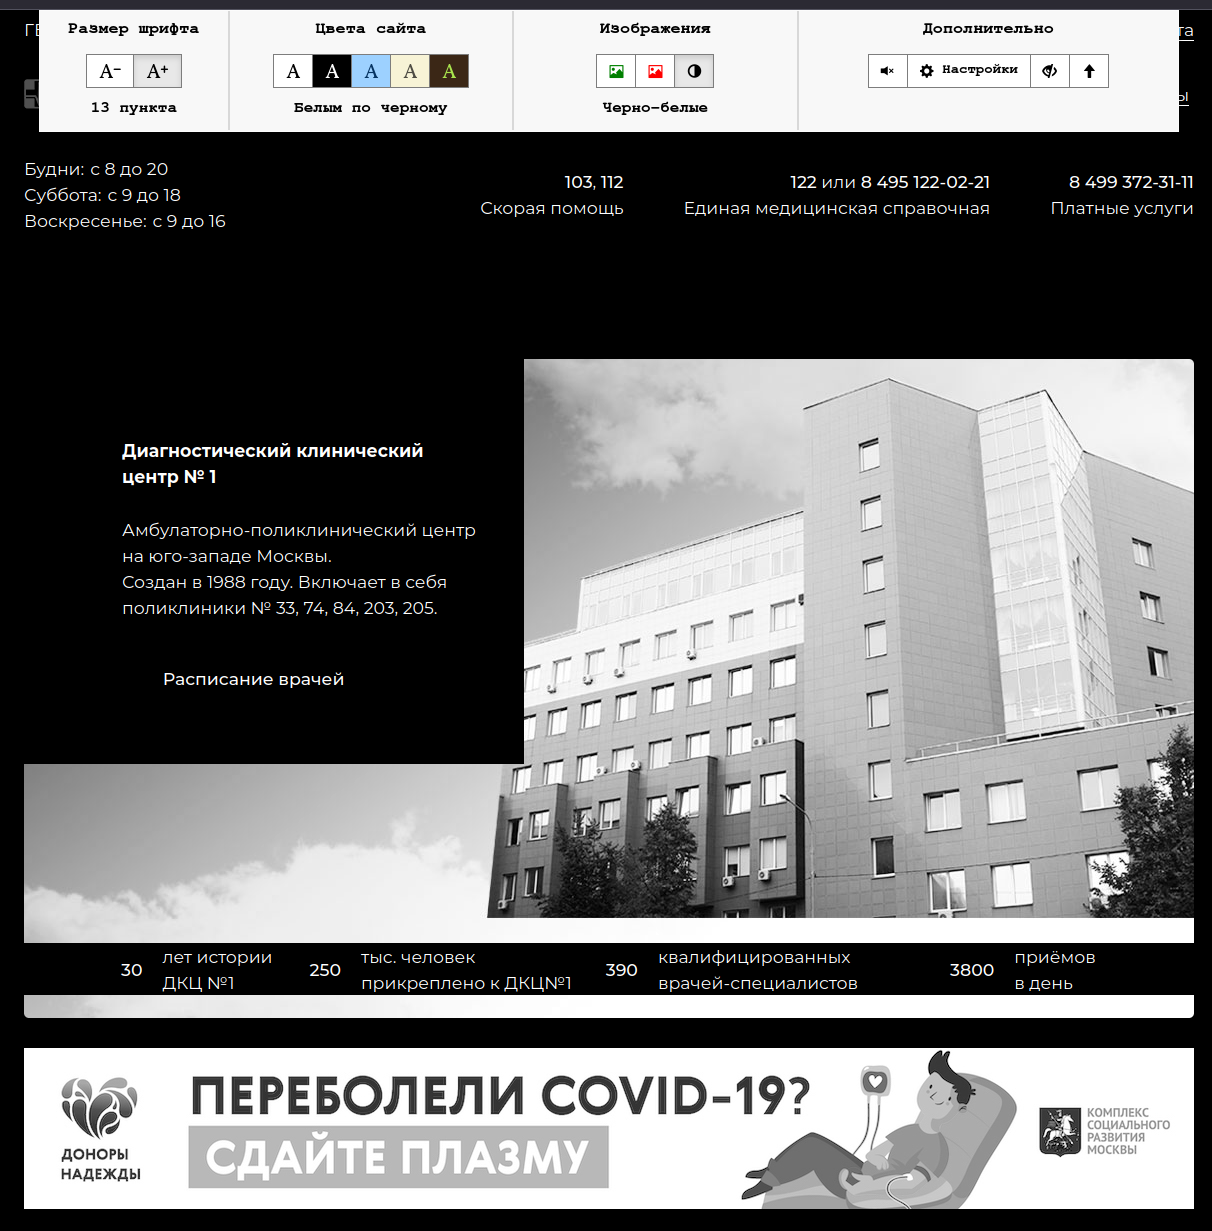
\includegraphics[width=\linewidth]{dkz2}}
    \captionof{figure}{дкц.рф версия для слабовидящих}
\end{minipage}
\bigskip

\noindent
\begin{minipage}{\linewidth}
    \fbox{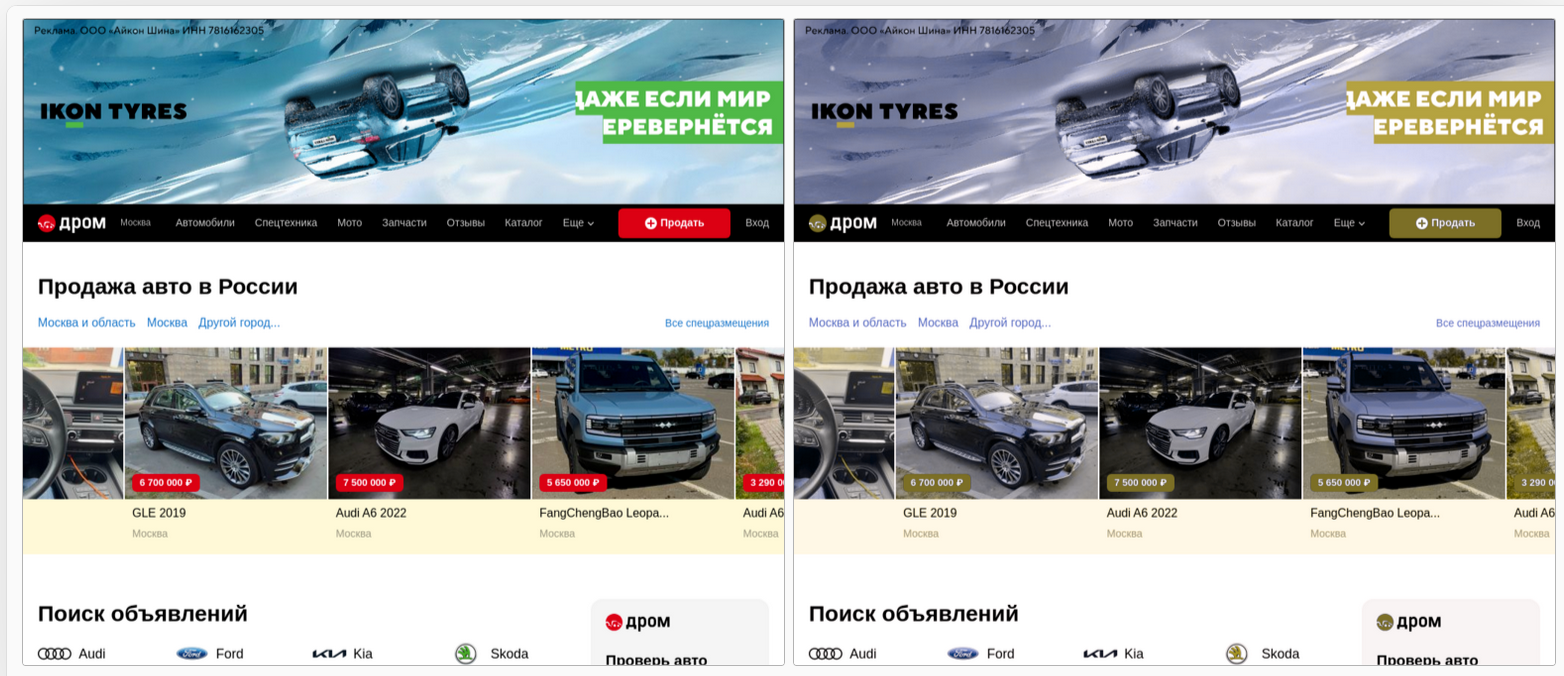
\includegraphics[width=\linewidth]{drom_protanopia}}
    \captionof{figure}{Протанопия drom.ru}
\end{minipage}
\bigskip

\noindent
\begin{minipage}{\linewidth}
    \fbox{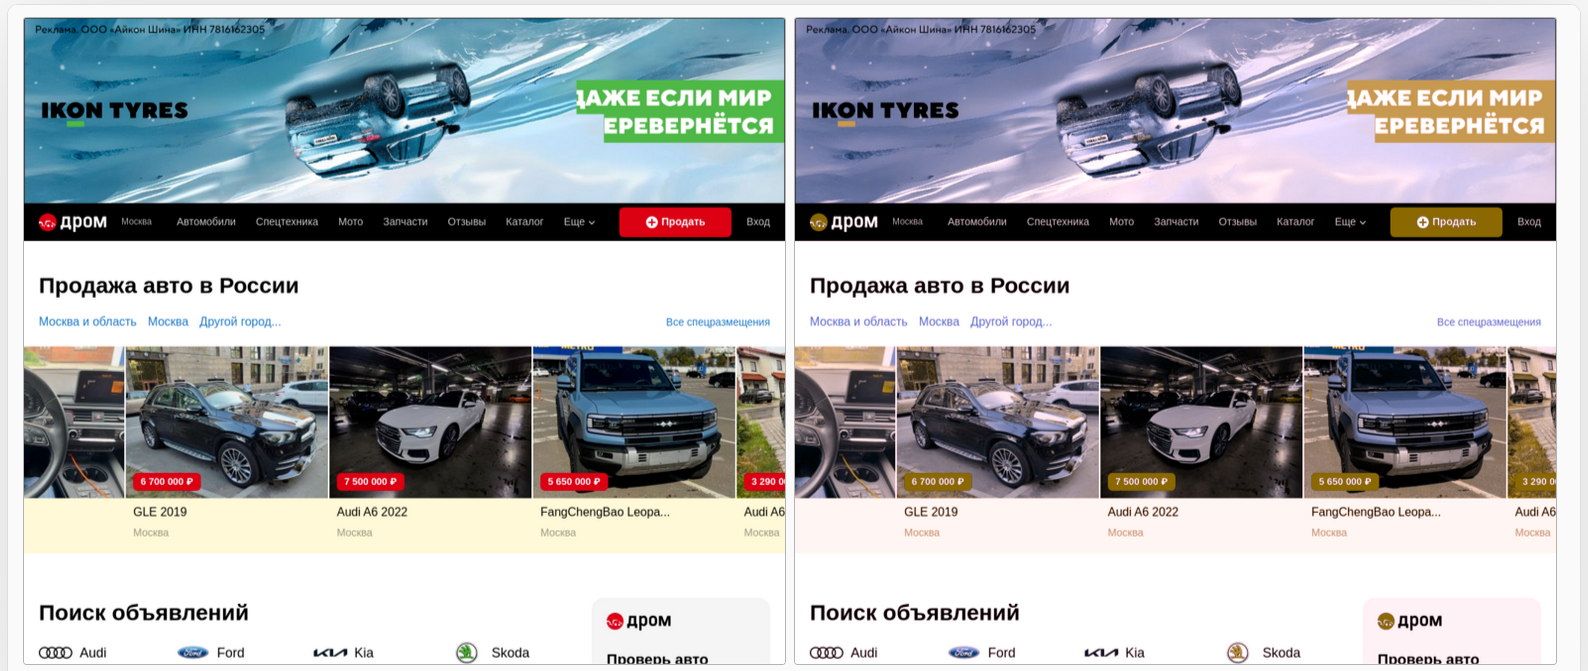
\includegraphics[width=\linewidth]{drom_deu}}
    \captionof{figure}{Дейтеранопия drom.ru}
\end{minipage}
\bigskip

\noindent
\begin{minipage}{\linewidth}
    \fbox{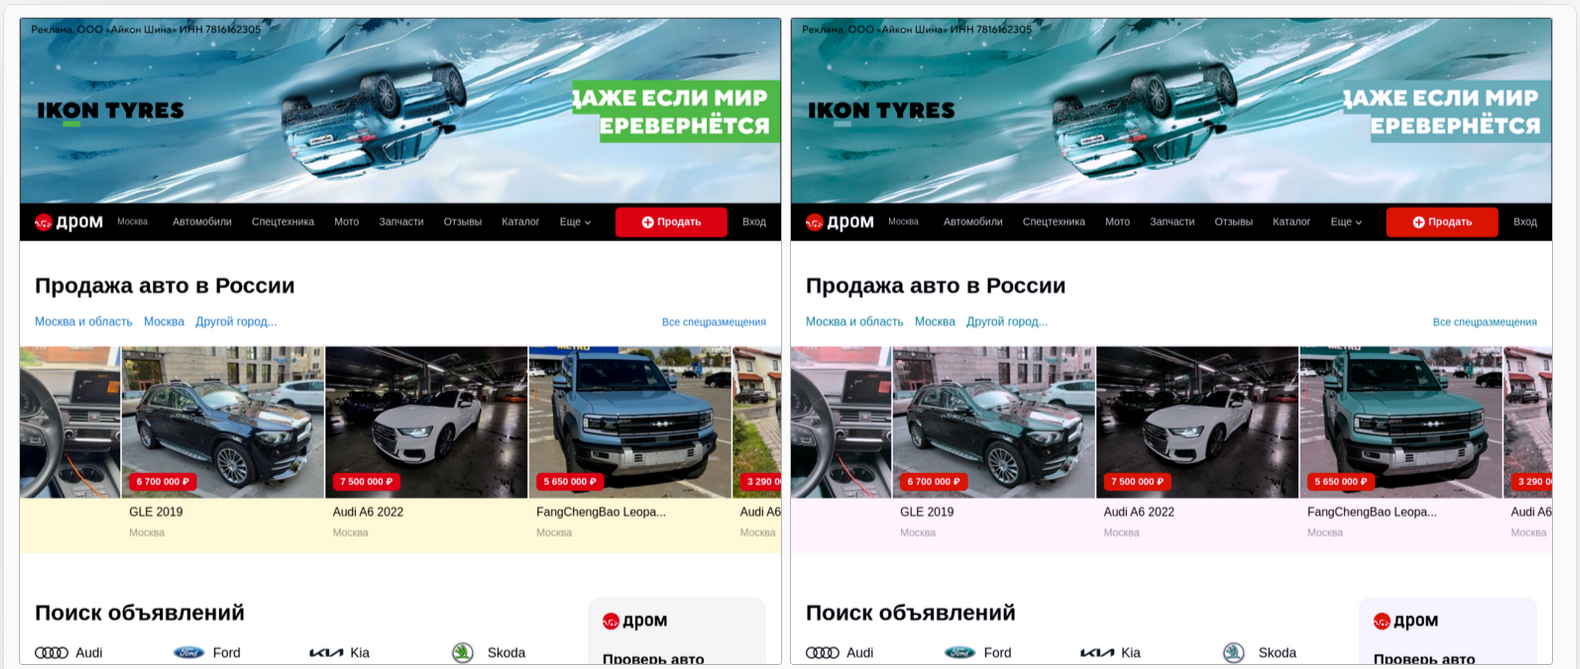
\includegraphics[width=\linewidth]{drom_tri}}
    \captionof{figure}{Тританопия drom.ru}
\end{minipage}
\bigskip

\noindent
\begin{minipage}{\linewidth}
    \fbox{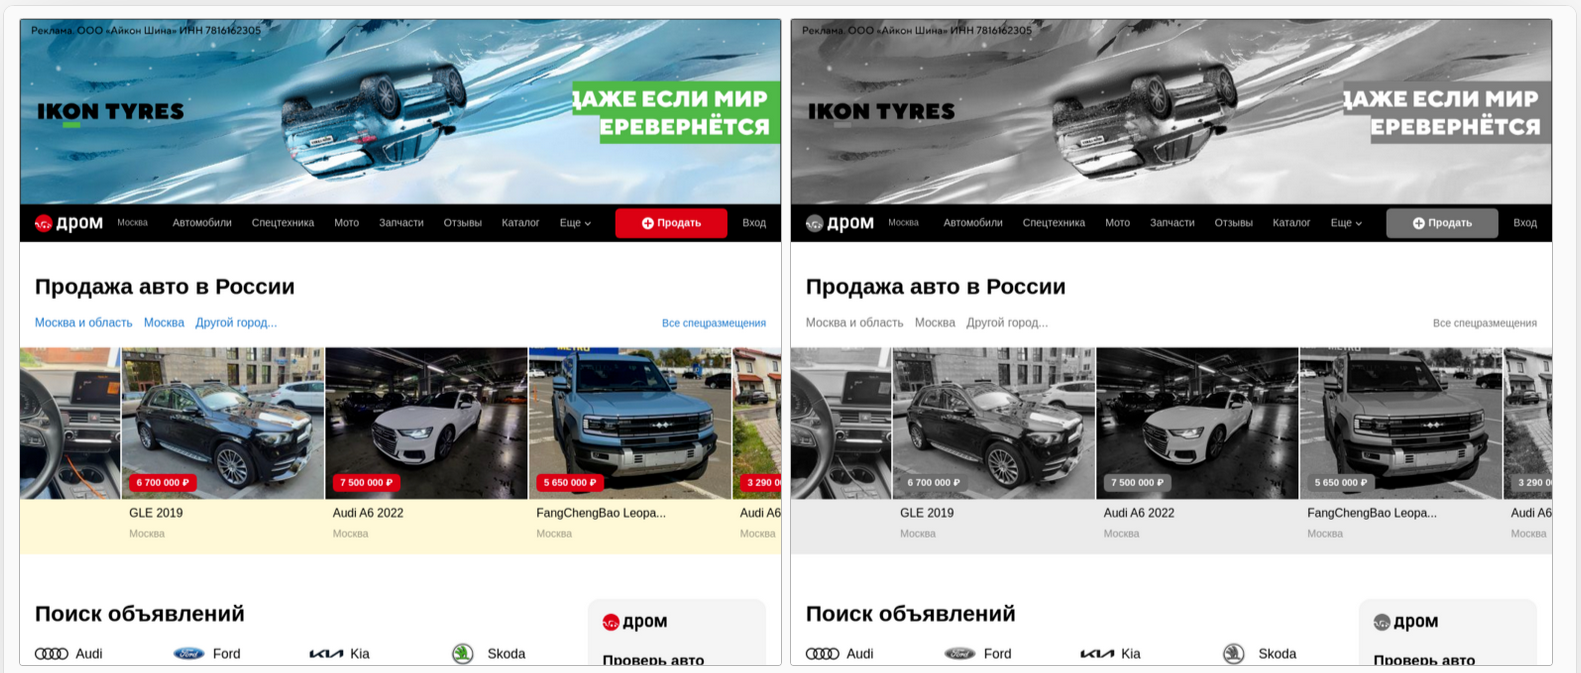
\includegraphics[width=\linewidth]{drom_ach}}
    \captionof{figure}{Ахроматопсия drom.ru}
\end{minipage}
\bigskip

\noindent
\begin{minipage}{\linewidth}
    \fbox{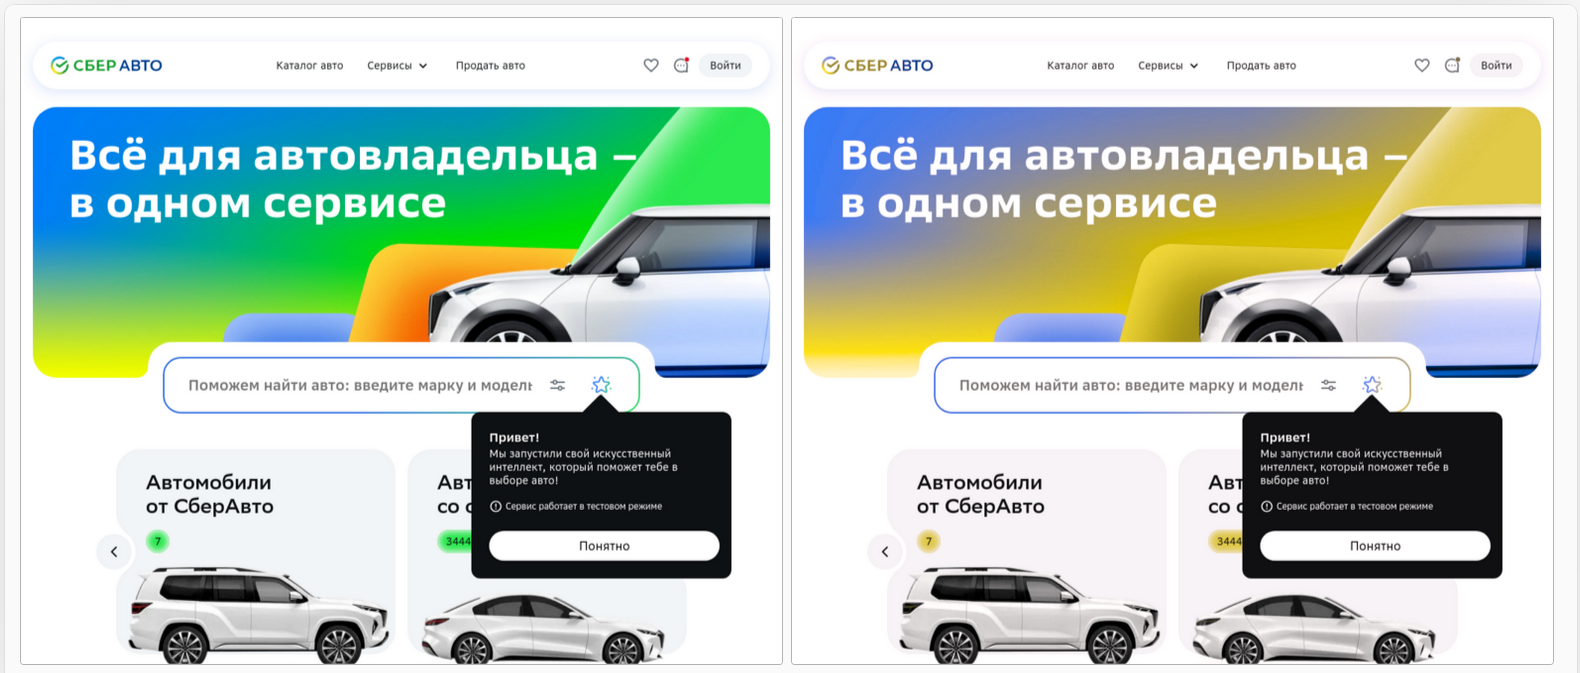
\includegraphics[width=\linewidth]{sber_protanopia}}
    \captionof{figure}{Протанопия sberauto.com}
\end{minipage}
\bigskip

\noindent
\begin{minipage}{\linewidth}
    \fbox{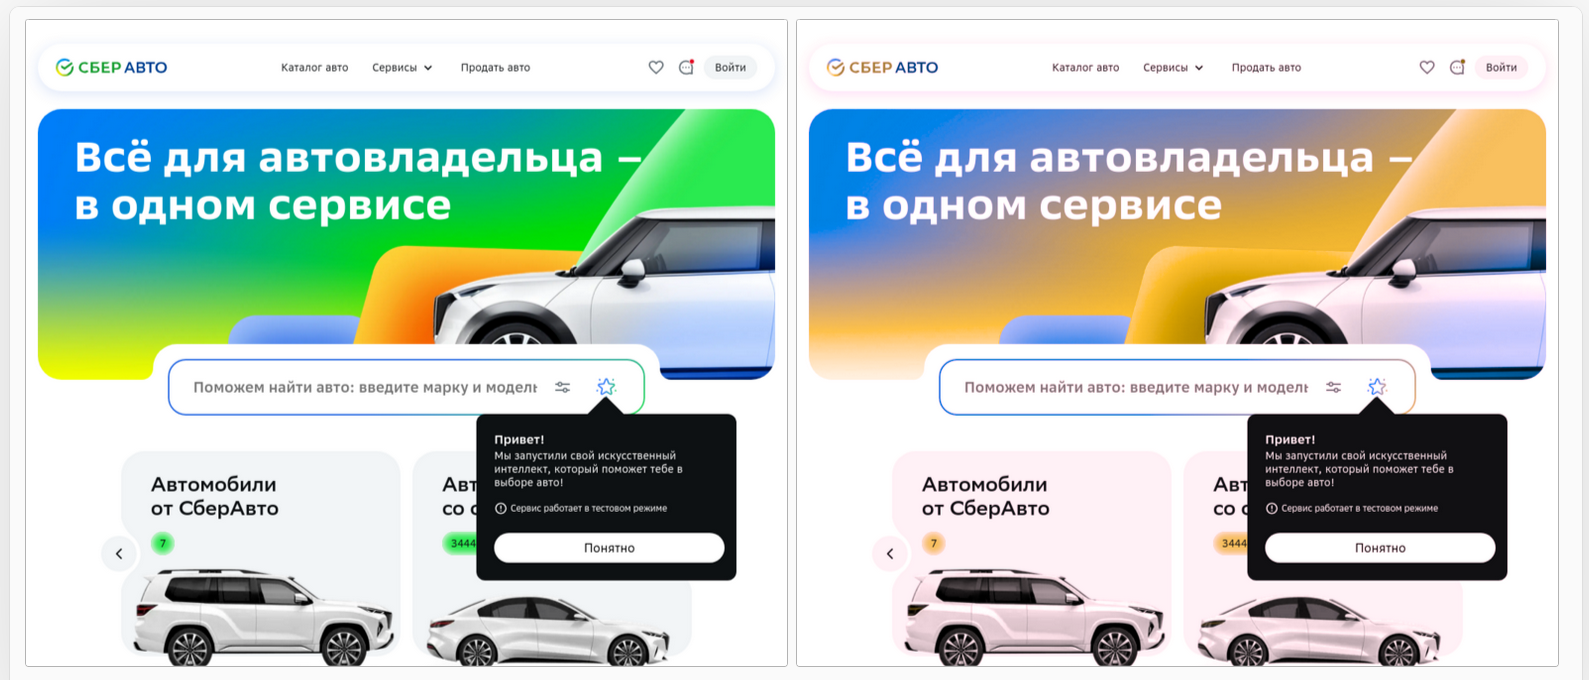
\includegraphics[width=\linewidth]{sber_deu}}
    \captionof{figure}{Дейтеранопия sberauto.com}
\end{minipage}
\bigskip

\noindent
\begin{minipage}{\linewidth}
    \fbox{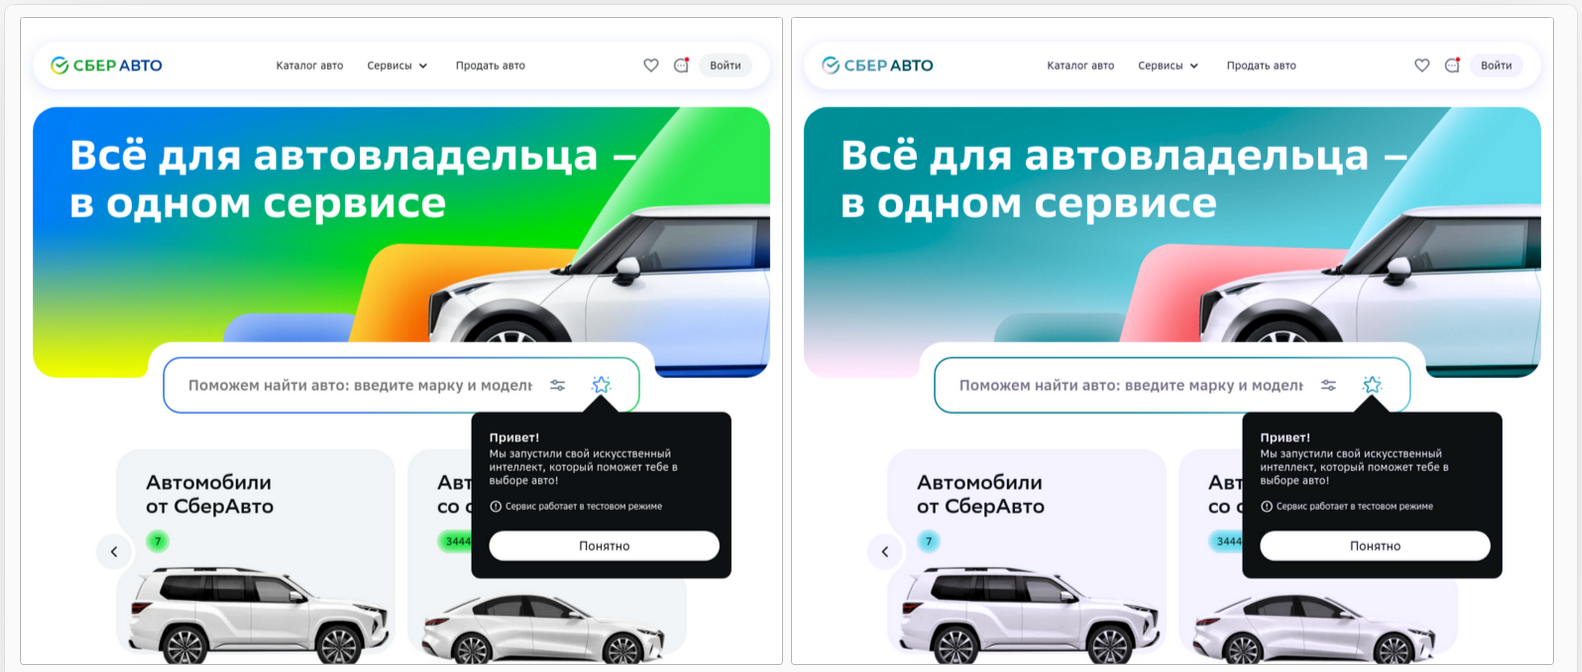
\includegraphics[width=\linewidth]{sber_tri}}
    \captionof{figure}{Тританопия sberauto.com}
\end{minipage}
\bigskip

\noindent
\begin{minipage}{\linewidth}
    \fbox{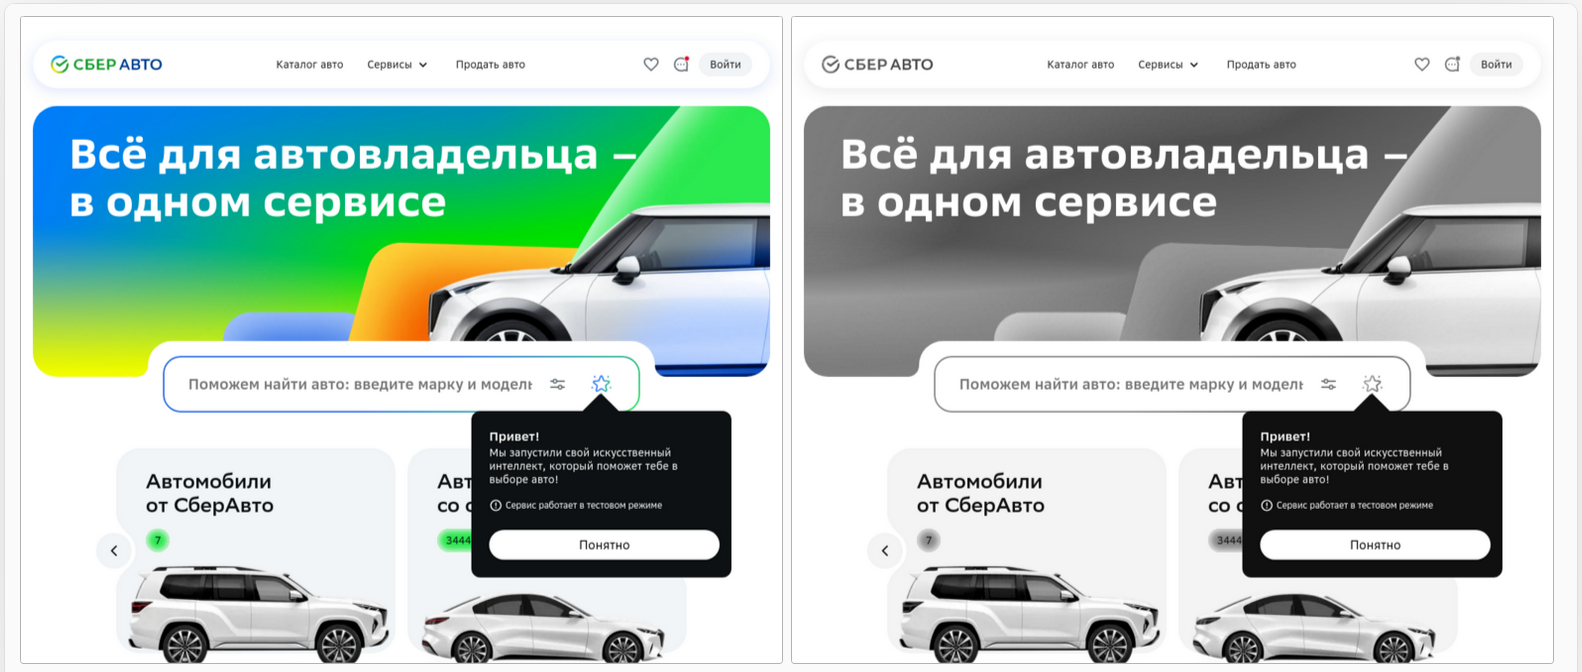
\includegraphics[width=\linewidth]{sber_ach}}
    \captionof{figure}{Ахроматопсия sberauto.com}
\end{minipage}
\bigskip

\noindent
\begin{minipage}{\linewidth}
    \fbox{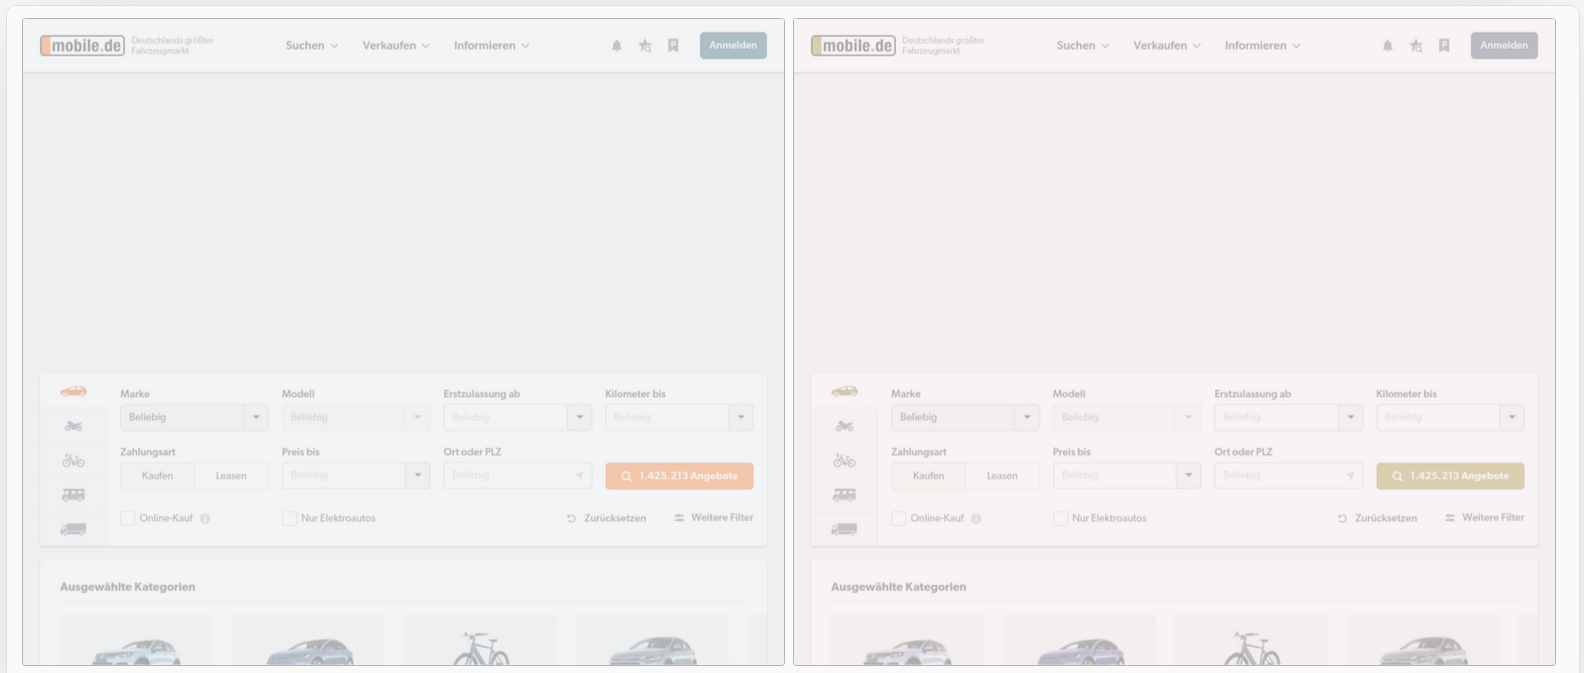
\includegraphics[width=\linewidth]{mobile_protanopia}}
    \captionof{figure}{Протанопия mobile.de}
\end{minipage}
\bigskip

\noindent
\begin{minipage}{\linewidth}
    \fbox{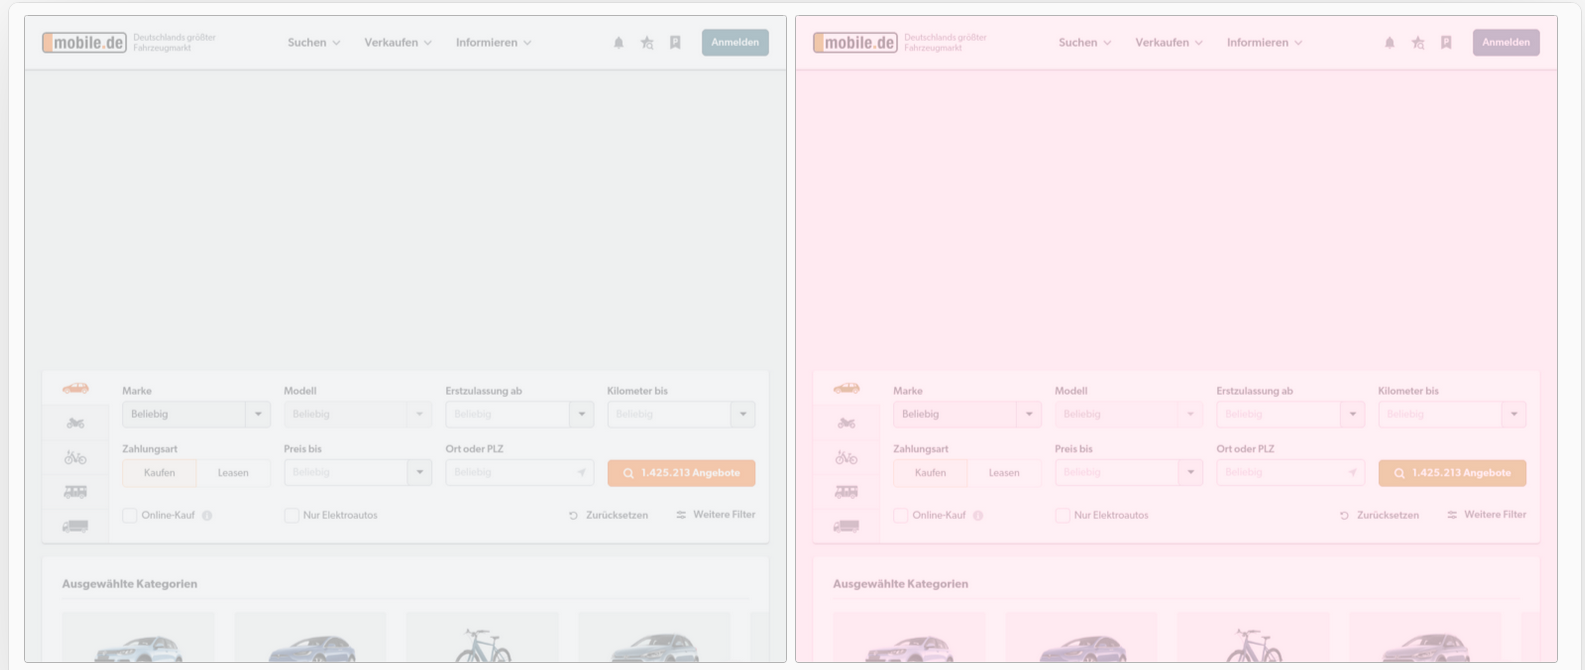
\includegraphics[width=\linewidth]{mobile_deu}}
    \captionof{figure}{Дейтеранопия mobile.de}
\end{minipage}
\bigskip

\noindent
\begin{minipage}{\linewidth}
    \fbox{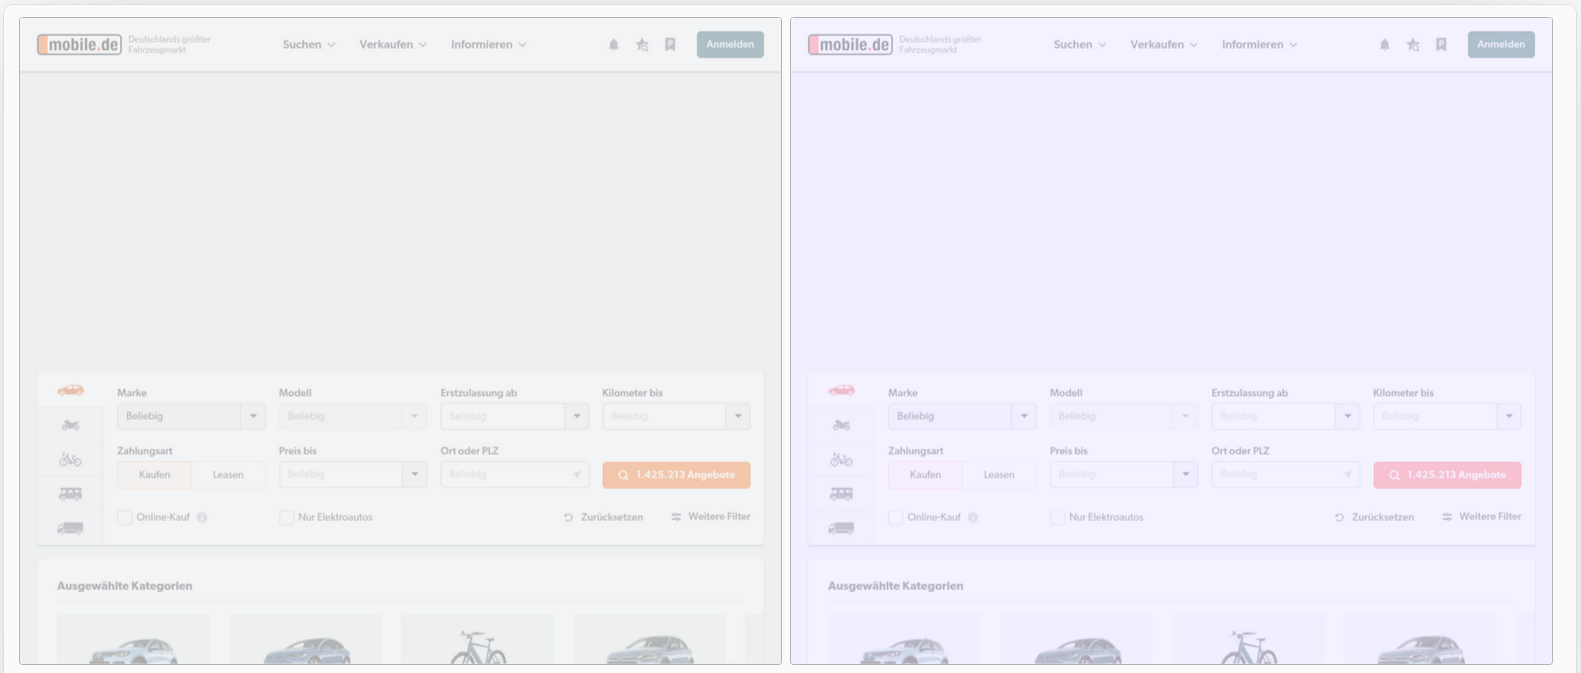
\includegraphics[width=\linewidth]{mobile_tri}}
    \captionof{figure}{Тританопия mobile.de}
\end{minipage}
\bigskip

\noindent
\begin{minipage}{\linewidth}
    \fbox{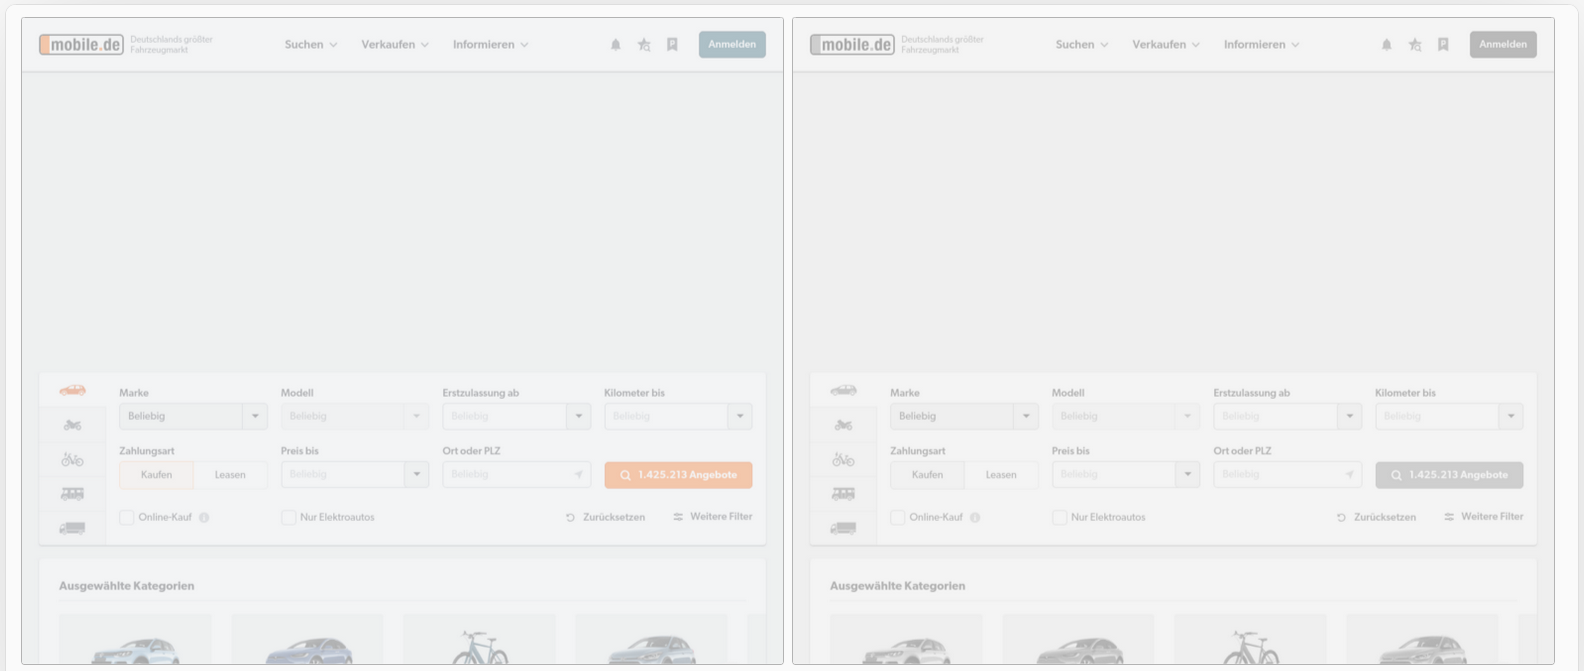
\includegraphics[width=\linewidth]{mobile_ach}}
    \captionof{figure}{Ахроматопсия mobile.de}
\end{minipage}
\bigskip

\noindent
\begin{minipage}{\linewidth}
    \fbox{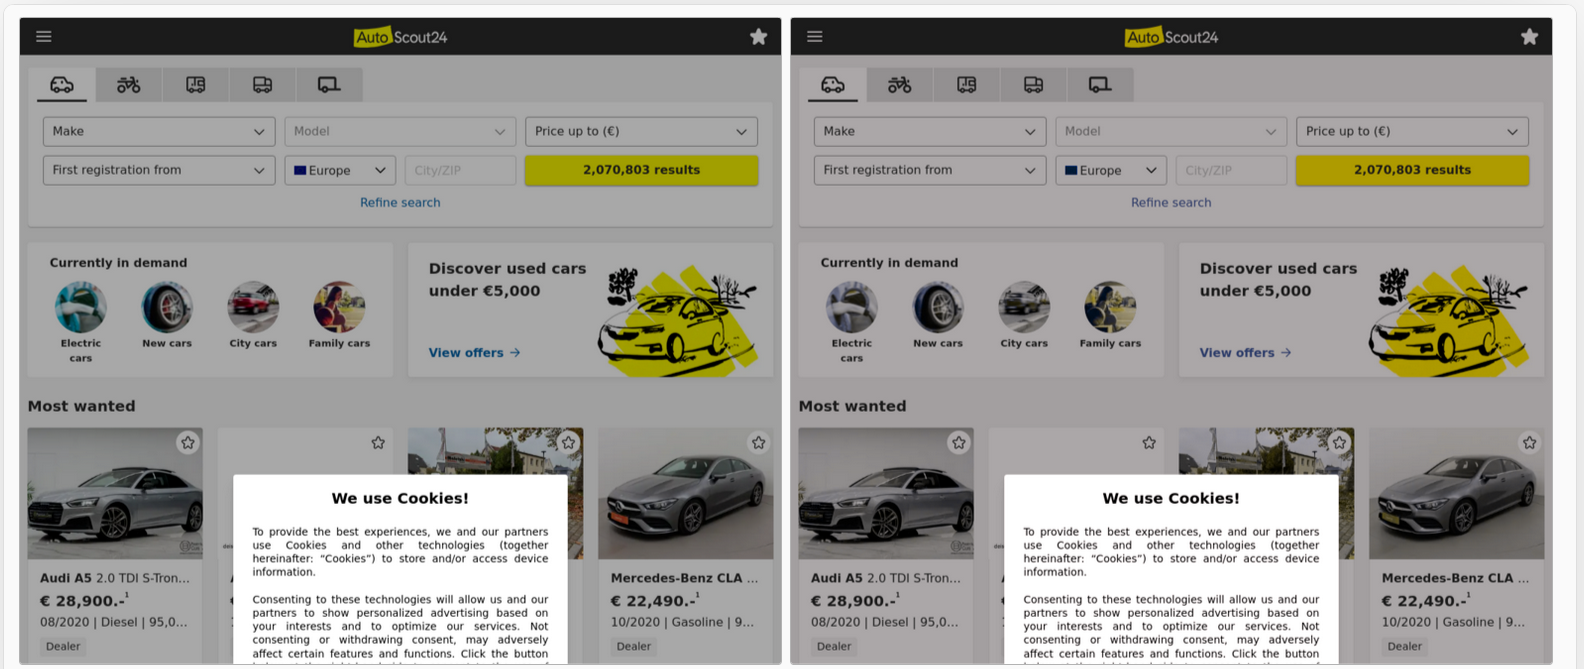
\includegraphics[width=\linewidth]{autoscout24_protanopia}}
    \captionof{figure}{Протанопия autoscout24.com}
\end{minipage}
\bigskip

\noindent
\begin{minipage}{\linewidth}
    \fbox{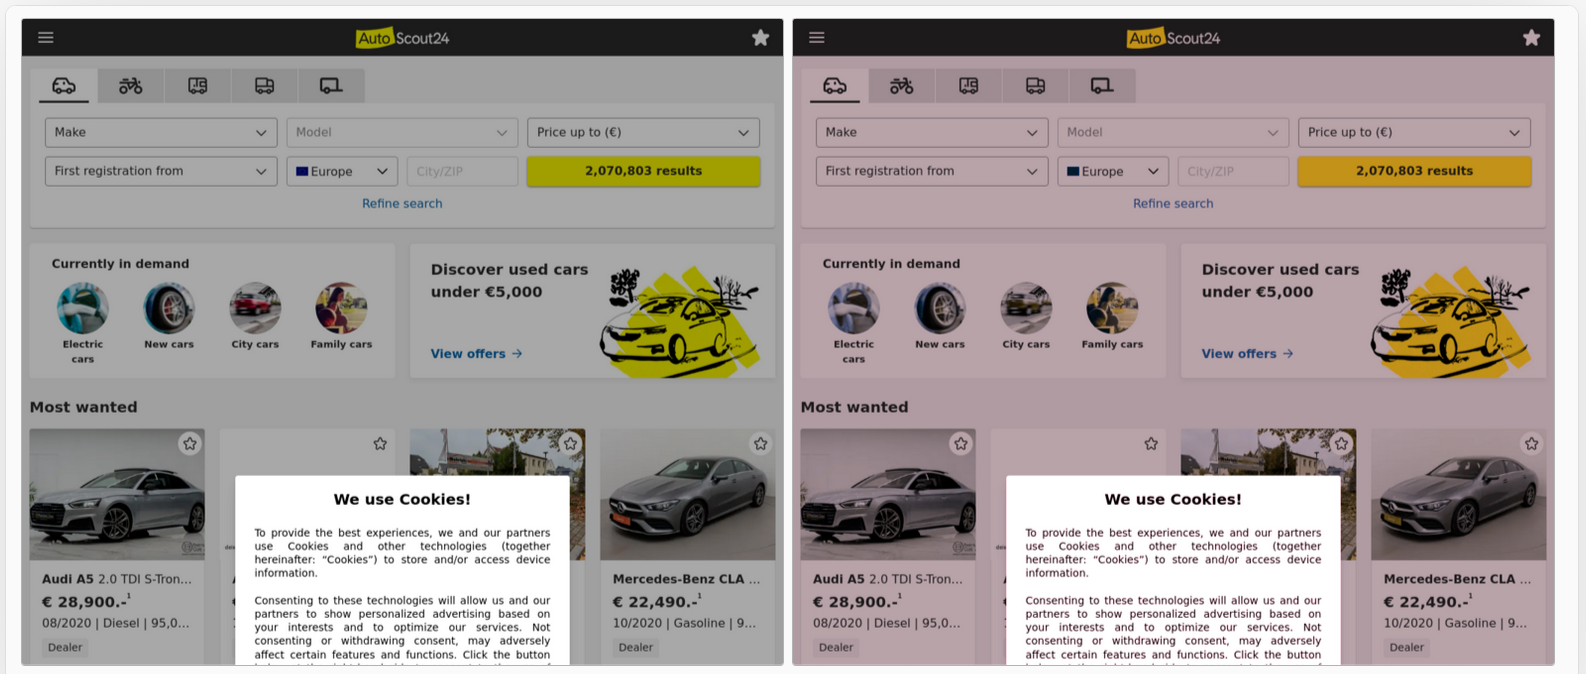
\includegraphics[width=\linewidth]{autoscout24_deu}}
    \captionof{figure}{Дейтеранопия autoscout24.com}
\end{minipage}
\bigskip

\noindent
\begin{minipage}{\linewidth}
    \fbox{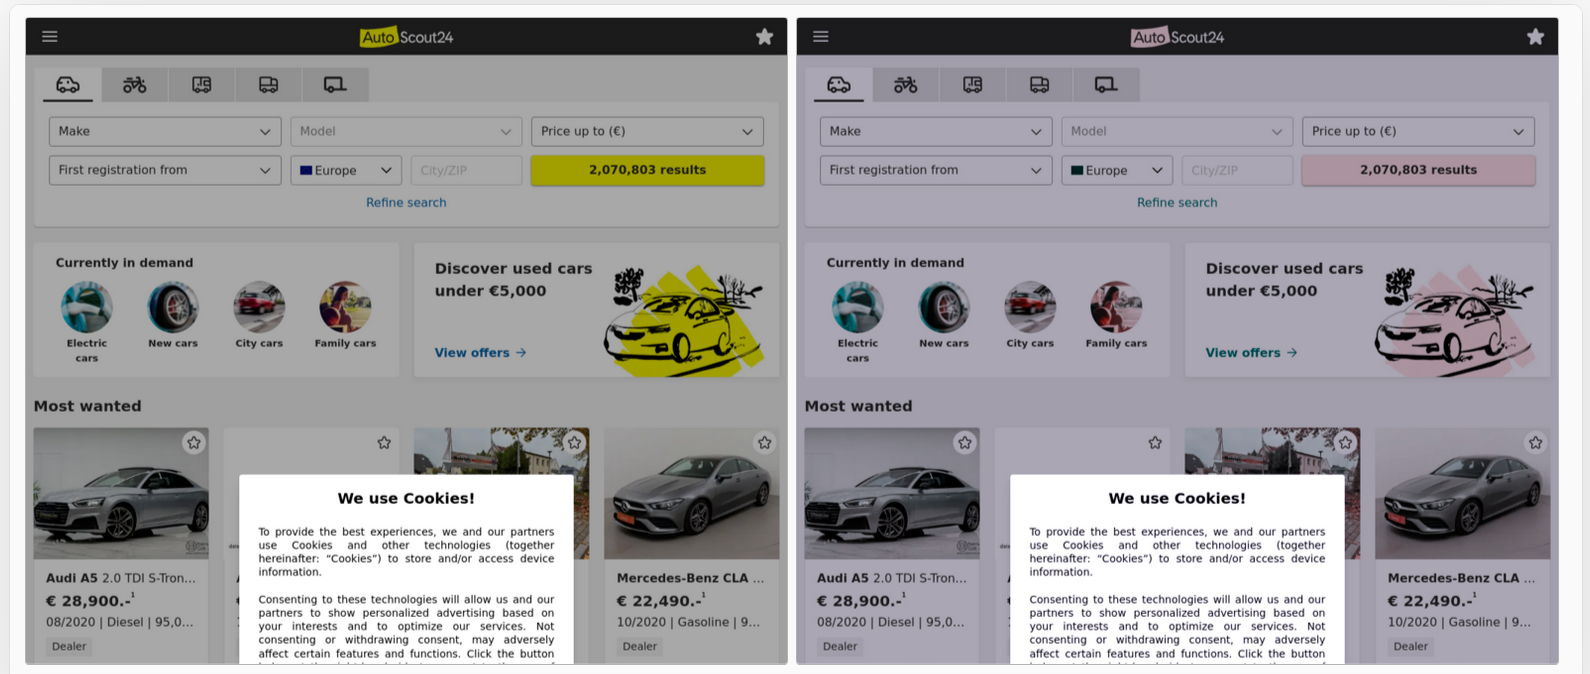
\includegraphics[width=\linewidth]{autoscout24_tri}}
    \captionof{figure}{Тританопия autoscout24.com}
\end{minipage}
\bigskip

\noindent
\begin{minipage}{\linewidth}
    \fbox{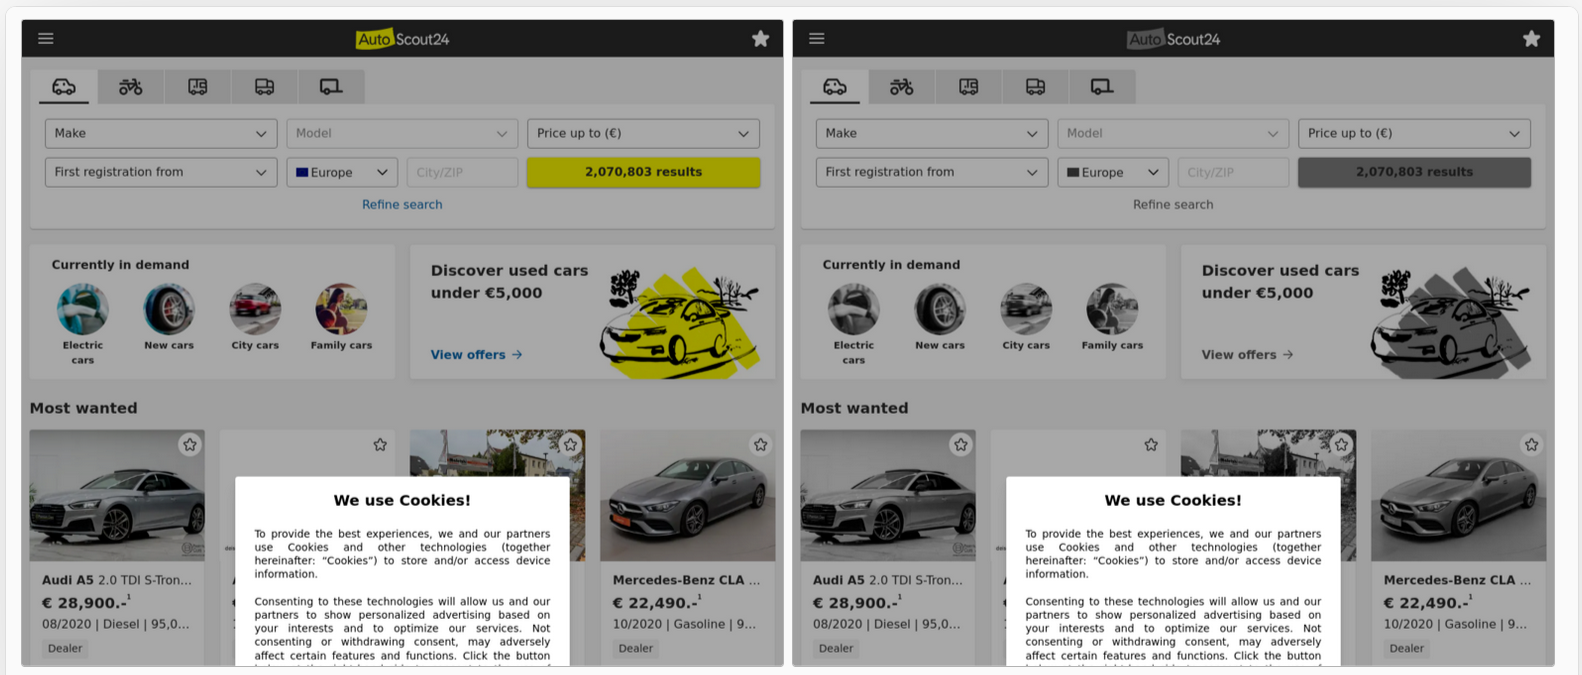
\includegraphics[width=\linewidth]{autoscout24_ach}}
    \captionof{figure}{Ахроматопсия autoscout24.com}
\end{minipage}
\bigskip

\noindent
\begin{minipage}{\linewidth}
    \fbox{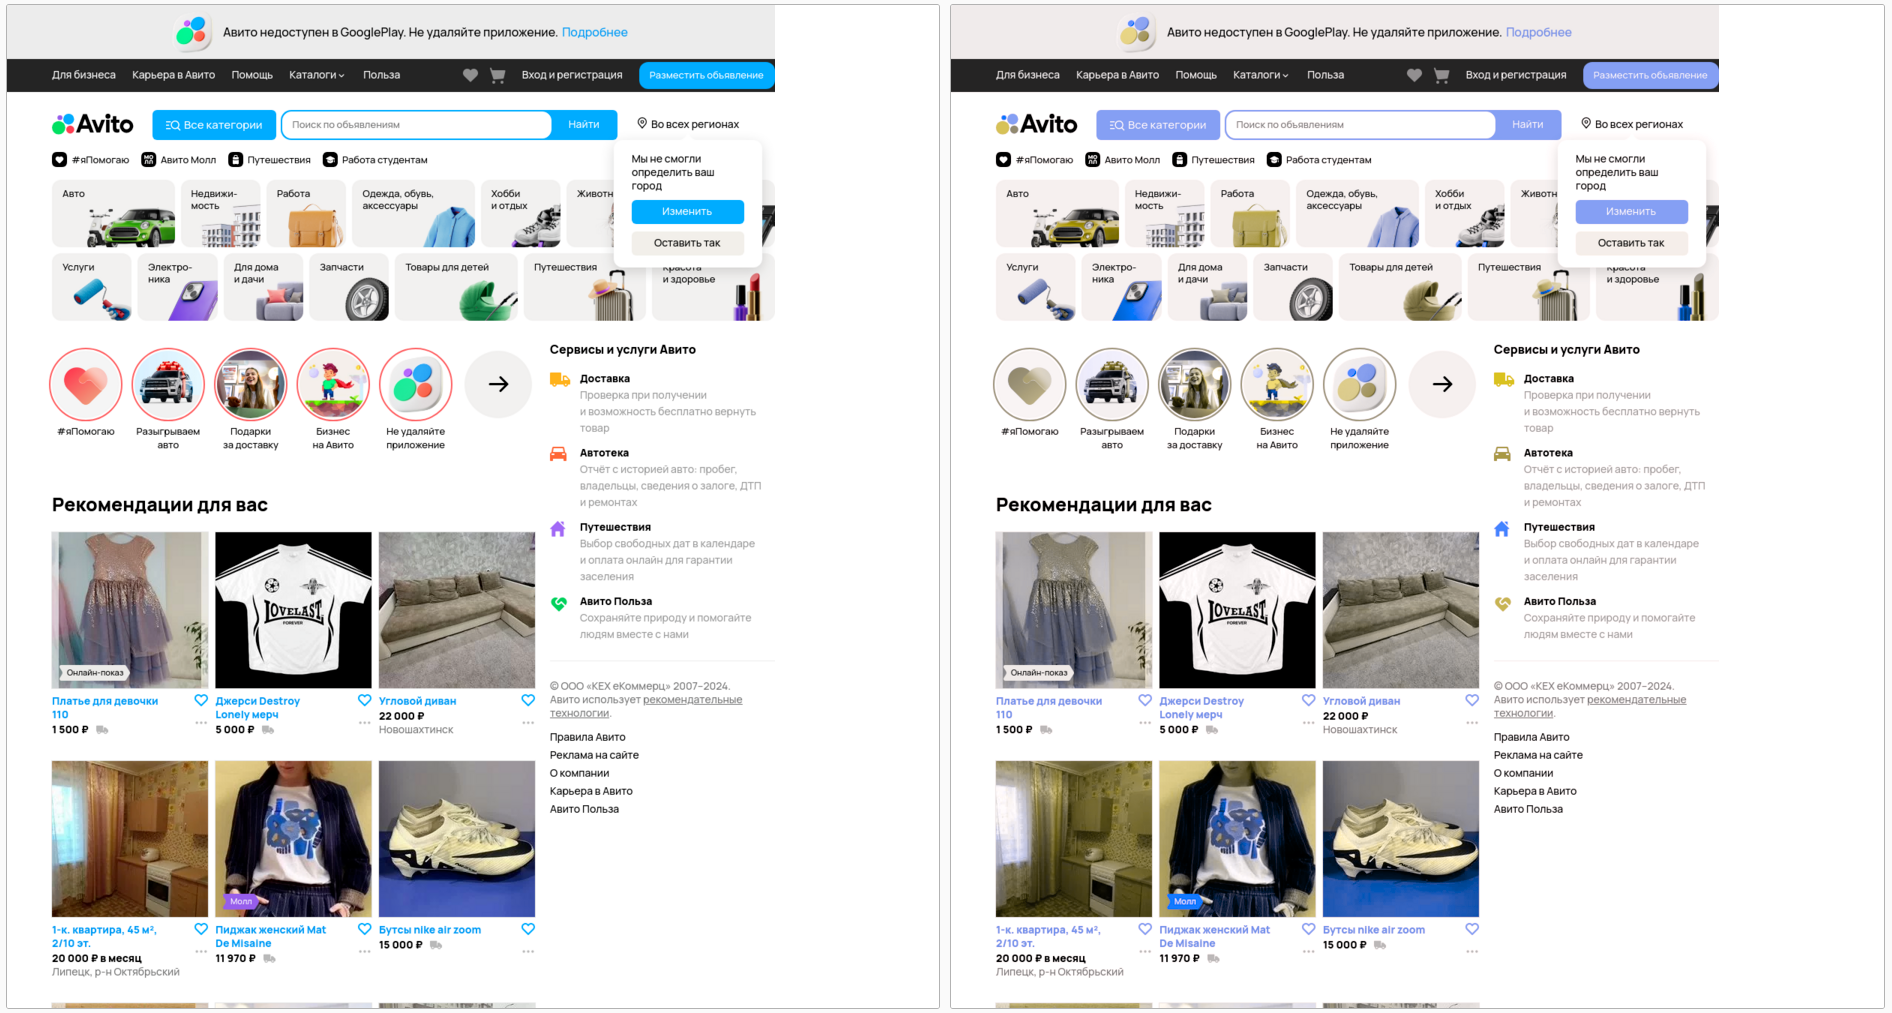
\includegraphics[width=\linewidth]{avito}}
    \captionof{figure}{Протанопия avito.ru}
\end{minipage}
\bigskip

\noindent
\begin{minipage}{\linewidth}
    \fbox{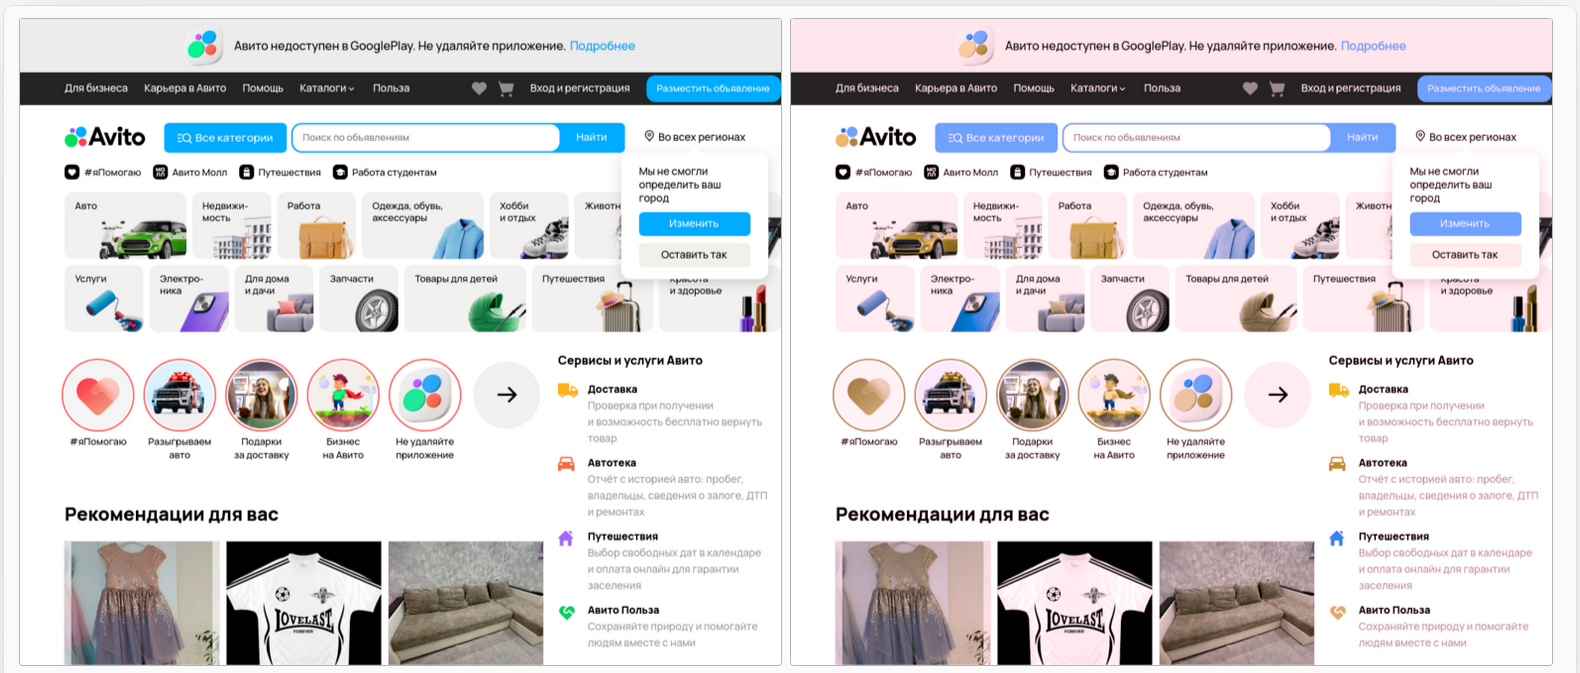
\includegraphics[width=\linewidth]{avito_deu}}
    \captionof{figure}{Дейтеранопия avito.ru}
\end{minipage}
\bigskip

\noindent
\begin{minipage}{\linewidth}
    \fbox{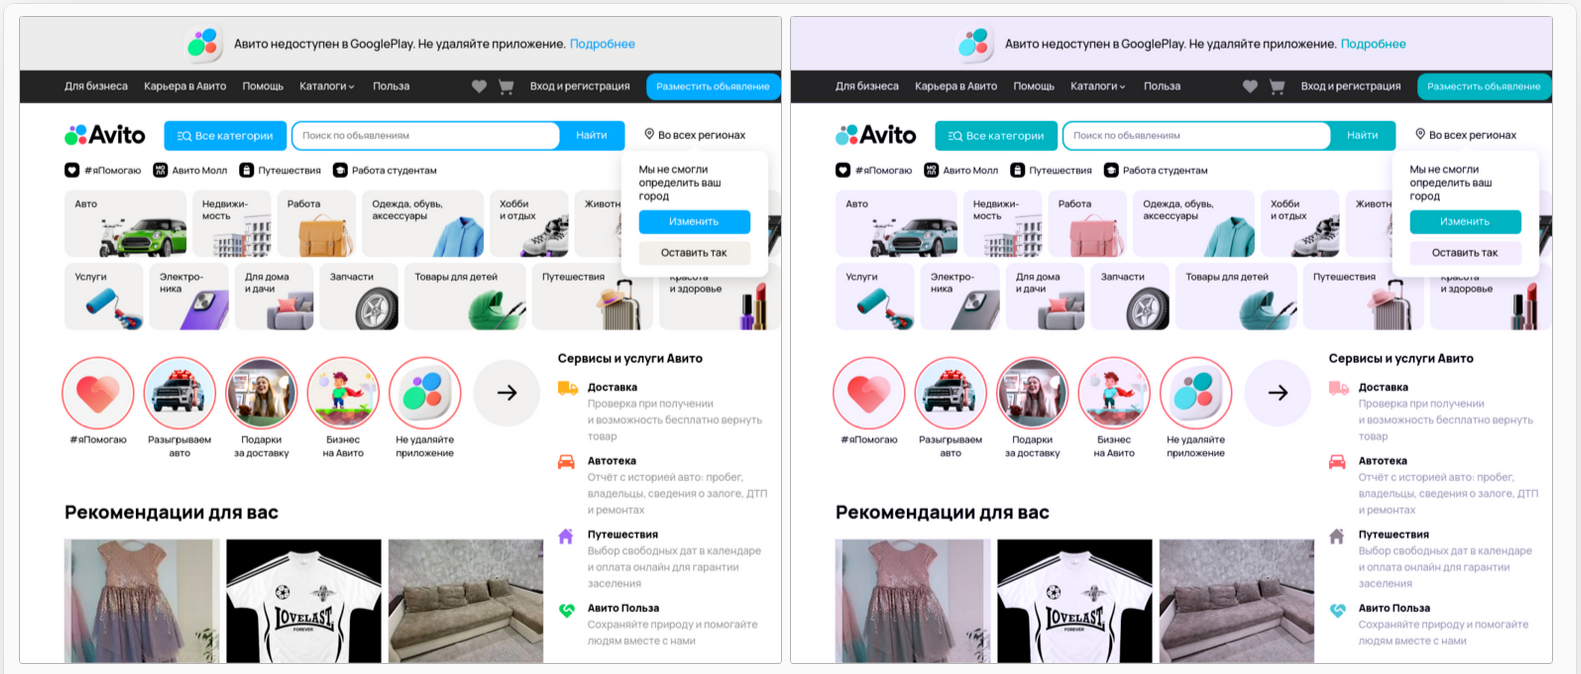
\includegraphics[width=\linewidth]{avito_tri}}
    \captionof{figure}{Тританопия avito.ru}
\end{minipage}
\bigskip

\noindent
\begin{minipage}{\linewidth}
    \fbox{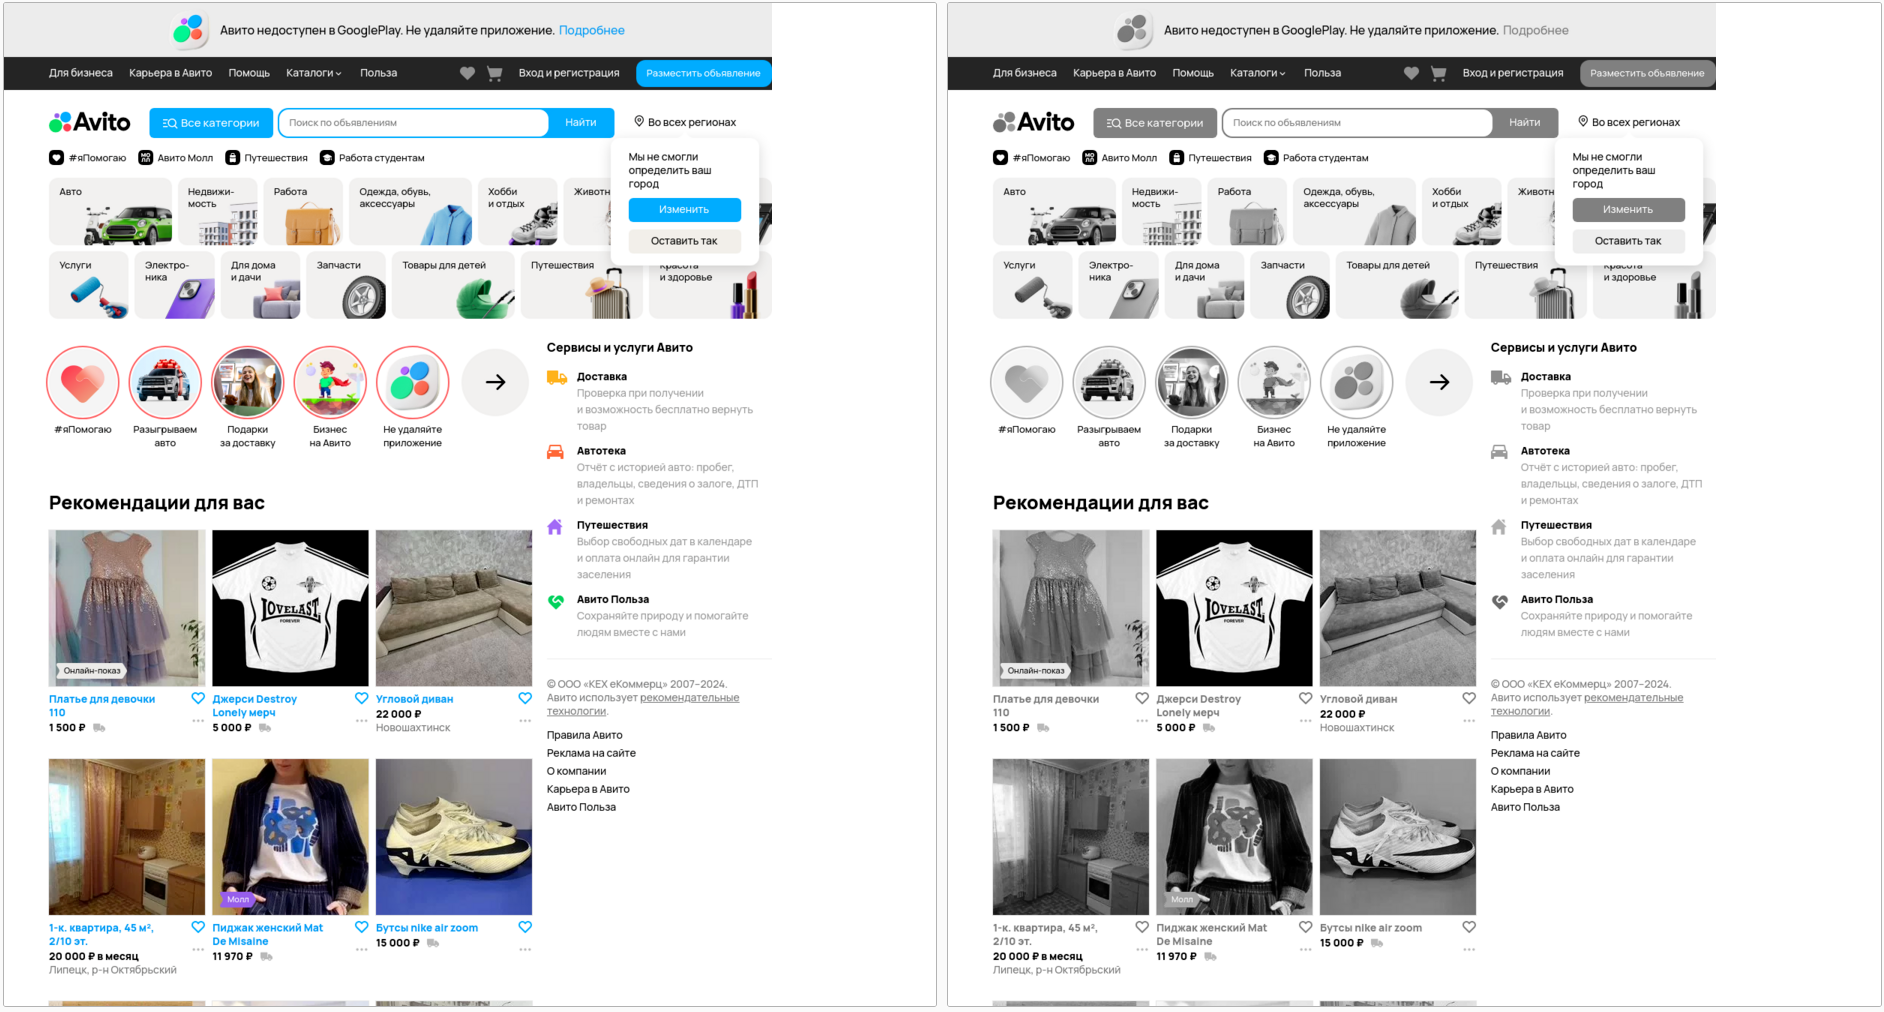
\includegraphics[width=\linewidth]{avito_gray}}
    \captionof{figure}{Ахроматопсия avito.ru}
\end{minipage}
\bigskip

\textbf{Контрольные вопросы и ответы}

\begin{enumerate}
    \item Какие аномалии цветового восприятия известны?

        Дальтонизм, Цветовая слабость, Ахроматопсия.
    \item Что такое цветовая слабость?

        Ослабленное восприятие определенного цвета (красного, зеленого или синего), при котором человек различает цвета, но с трудом и нечетко, из-за частичной дисфункции колбочек в глазу. Это состояние встречается чаще, чем цветовая слепота, и требует повышенного внимания к выбору контрастных цветовых схем при проектировании интерфейсов.
    \item Что такое цветовая слепота ?

         Полное отсутствие восприятия одного из основных цветов (красного, зеленого или синего) из-за дефекта или отсутствия одного из типов колбочек. Люди с цветовой слепотой видят меньше цветовых оттенков, чем люди с нормальным зрением, и могут путать определенные цвета, особенно при недостаточной контрастности.
    \item Какие существуют рекомендации (правила) по дизайну интерфейсов, которые помогут людям с нарушениями цветовосприятия остаться на  сайте?

        Обеспечивать высокую контрастность. Для выделения информации вместо одного только цвета использовать текстуры и формы. Минимизировать цветовую палитру. Избегать градиентов, во избежании затруднения восприятия.
    \item Как аномалии цветового восприятия учитываются при проектировании веб-ресурсов? Каких базовых правил рекомендуется придерживаться?

        При проектировании сайтов важно учитывать, что пользователи с аномалиями цвета различают цвета по яркости и контрасту. Важно избегать проблемных сочетаний, таких как красный и зеленый, розовый и серый, фиолетовый и синий. Для этого используют симуляторы для проверки интерфейса и корректируют цветовую палитру в зависимости от результатов тестирования.
    \item Что регламентирует международный стандарт Web Content Accessibility Guidelines (пер. «Руководство по доступности веб-материалов») WCAG?

        WCAG определяет международные рекомендации по обеспечению доступности веб-контента для людей с ограниченными возможностями, включая тех, у кого есть нарушения цветового восприятия. Стандарт описывает методы повышения контрастности текста, использования альтернативных методов визуальной передачи информации (например, текстур и символов) и соблюдения минимального уровня контрастности для текстовых и графических элементов.
\end{enumerate}

\end{document}
